

\chapter{Исчисление остатков}\label{ostatki}

\vrezka{
Арифметика остатков дает богатый фактологичекий материал для изучения свойств простых чисел, а также позволяет по-новому взглянуть на операции Минковского с числовыи множествами и выйти на такие важные вехи теории множеств, как виды отношений и фактормножества.
}

\section{Арифметика остатков}

\subsection*{Конспект}
\begin{enumerate}\setlength{\itemsep}{1pt}
\item Рассмотрим бытовую задачу. Вам нужно выключить печку через 40 минут, но у вас нет таймера, зато есть будильник, на котором можно выставить время звонка. Сейчас 12:30, на какое время требуется поставить будильник? Ответ: 13:10. Почему так? Дело в том, что в часе 60 минут, и если к 30 минутам прибавить 40, получается 70 минут, что больше часа. Поэотму добавляем 1 час и остаток --- 10 минут.
\item Еще пример: сколько часов будет через 20 часов, если сейчас 8 утра? Можно решать аналогично: $8+20=28$, затем убираем полные сутки, т.е. 24 часа, остается 4 часа утра.
\item Можно решать иначе. 20 часов --- это $-4$ часа от суток. Следовательно, нужно просот вычесть из 8 утра 4 часа и получим те же 4 часа утра.
\item Во всех случаях мы решаем задачу нахождения остатка от деления на некоторое число. В случае минут это 60, в случае часов это 24.
\item Когда вас просят отметить в анкете количество полных лет, то вам по сути нужно найти неполное частное от деления вашего возраста на 1 год. Конечно, в данном случае нам это просто сделать, т.к. каждый год мы запоминаем именно количество прожитых лет, а не дней или недель.
\item Но, например, во многих сферах деятельности планирование календаря происходит неделями (и даже у себя в компьютере в настройках календаря вы можете вывести номер текущей недели в году). А сколько недель в году? Для этого нужно найти неполное частное от деления 365 (или 366) на 7, оно составляет 52.
\item Остаток от деления на неделю есть число от 0 до 6, которое определяет сдвиг вперед относительно текущего дня недели. Например, если сегодня четверг, то какой день недели будет через 30 дней? Мы выбрасываем из 30 4 полных недели, что составляет 28 дней, и находим остаток, который равен 2. Это значит, что через 30 дней будет четверг плюс 2 дня, т.е. суббота.
\item Точно так же можно легко заметить, что каждый год происходит смещение дат на 1 или два дня вперед относительно дней недели. Так, если в этом году 1 января было средой, то в следующем оно будет или четвергом (если мы не переходим через 29 февраля), или пятницей (если текущий год --- високосный, т.е. содержит 366 дней), как на картинке ниже.

\begin{center}
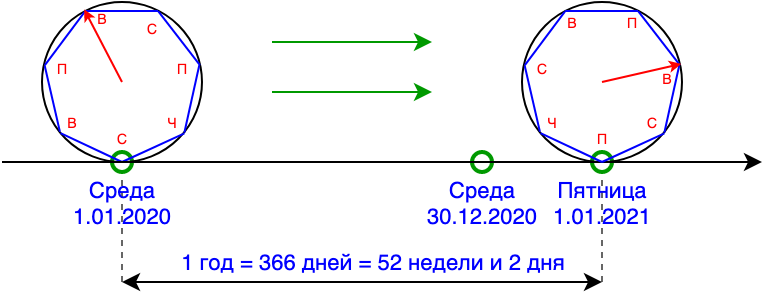
\includegraphics[scale=0.4]{weekdays.png}
\end{center}

\item Каждые 28 лет (а 28 --- это наименьшее общее кратное 7 и 4) соответствие дат и дней недели повторяется.
\item При расчетах на более длительные периоды, а именно, при переходе через 1900 год или 2100 год, нужно учитывать также, что 3 раза за 400 лет не происходит добавление лишнего дня (29 февраля) для более точного соответствия календаря астрономическому году, т.е. 1900, 1800, 1700 годы не являются високосными, как и 2100, 2200 и 2300.
\item Тем не менее, часто в жизни встречается задача вычисления дня недели, и здесь нам на помощь приходит исчисление остатков по модулю 7. Например, сегодня 21 марта 2020 суббота, а нам нужно знать, какой день недели будет 31 августа 2020. Сначала мы находим день недели 21 августа, т.к. до этой даты целое число месяцев. При этом мы 3 раза переходим через 31 число (март, май, июль) и 2 раза --- не переходим (апрель, июнь). Следовательно, 3 раза прибавляется остаток 3, и 2 раза --- остаток 2, итого сумма остатков составляет 13. Но это больше 7, причем очень близко к 14, поэтому сумму остатков мы запишем как -1. Наконец, остается добавить 10 дней (от 21 августа до 31 августа). Итого получается 9, а по модулю 7 --- всего 2. Таким образом, 31 августа 2020 года есть понедельник!
\item Из приведенной выше картинки с семиугольником на окружности, совмещенной с прямой линией, мы можем ясно представить себе, как работает исчисление остатков по модулю 7, т.е. исчисление дней недели. Мы катим окружность по прямой времени, пока не достигнем нужной нам даты. При этом неважно, сколько целых оборотов совершит семиугольник, т.е. сколько недель мы проедем, а вот последний полувиток как раз и дает нам ответ на вопрос о дне недели. Так что, если мы пронумеруем дни недели цифрами от 0 до 6, то любое расстояние между датами можно представить как какое-то целое количество недель плюс остаток, лежащие в диапазоне от 0 до 6 (включительно).
\item Эта картинка легко обобщается на случай произвольного основания. Представим, что в неделе у нас не 7 дней, а, например, 28 (лунный месяц), и тогда любое расстояние между датами выражается как целое число 28-дневных циклов плюс некоторый остаток от 0 до 27. И так далее.
\item Таким образом, мы приходим к тому, что всякое натуральное число (количество) можно представить в виде $a=km+b$, где $k$ --- неполное частное от деления $a$ на $m$, $b$ --- остаток от деления, который находится в промежутке от 0 (включая) до $m$ (не включая).
\item Равенство $a=km+b$ при исчислении остатков принято записывать так:
$$
a\equiv b\pmod m,
$$
Читается: $a$ сравнимо с $b$ по модулю $m$.

Причем, если модуль $m$ известен из контекста и не меняется при вычислениях, то его можно опускать, записывая просто $a\equiv b$. Читается: $a$ \textbf{сравнимо с} $b$ (по модулю $m$).

\item На картинке, приведенной выше, даты 1 января 2020 и 30 декабря 2020 сравнимы по модулю 7, т.е. по дням недели.
А про интервал в 366 дней мы запишем $366\equiv 2\pmod 7$. Такая запись никак не информирует нас о коэффициенте $k$ (количестве целых недель), но показывает самое главное --- сколько дней надо прибавить к среде.
\item Остатками можно оперировать так же, как обычными числами, сбрасывая всякий раз накопленные при сложении целые <<оброты>> модулей. Иначе говоря, если мы хотим, например, к текущей среде прибавить 6 дней, то мы совмещаем наш семиугольник вершиной <<среда>> с прямой времени, а затем прокатываем его вперед на 6 делений (что чуть меньше полного оборота), и в точке касания с прямой получаем вторник. Заметим, что ровно тот же результат мы получим, если прокатим семиугольник назад на 1 деление. Это значит, что числа 6 и -1 сравнимы по модулю 7. И на практике можно также пользоваться отрицательными числами для исчисления остатков.
\item Ранее мы много времени уделяли таблицам композиций движений многоугольников. И, как мы помним, композиция вращений многоугольника соответствовала сложению углов этих вращений. При этом мы также отбрасывали 360 градусов (или $2\pi$), если сумма углов переваливала за полный оборот. При описании конечных подгрупп движений правильных многоугольников мы выяснили, что каждый поворот является степенью некоторого минимального поворота на угол $2\pi/n$ (для $n$-угольника), т.е. все повороты выражаются углами $k(2\pi/n)$, где $k=0,\dots,n-1$ (ничего не напоминает?).
\item Забудем теперь про вращения и углы, а просто понаблюдаем за степенями этих поворотов при композициях, т.е. при сложении углов. Для примера рассмотрим случаи $n=7$ и $n=8$, и выпишем таблицу композиций, которая представлят собой таблицу сложения остатков по модулям 7 и 8, соответственно.
\item Таблицы сложения остатков по модулям 7 и 8:
\begin{center}
\begin{tabular}{c||c|c|c|c|c|c|c|}
  & 0 & 1 & 2 & 3 & 4 & 5 & 6 \\ \hline\hline
0 & 0 & 1 & 2 & 3 & 4 & 5 & 6 \\ \hline
1 & 1 & 2 & 3 & 4 & 5 & 6 & 0 \\ \hline
2 & 2 & 3 & 4 & 5 & 6 & 0 & 1 \\ \hline
3 & 3 & 4 & 5 & 6 & 0 & 1 & 2 \\ \hline
4 & 4 & 5 & 6 & 0 & 1 & 2 & 3 \\ \hline
5 & 5 & 6 & 0 & 1 & 2 & 3 & 4 \\ \hline
6 & 6 & 0 & 1 & 2 & 3 & 4 & 5 \\ \hline
\end{tabular}
\quad
\begin{tabular}{c||c|c|c|c|c|c|c|c|}
  & 0 & 1 & 2 & 3 & 4 & 5 & 6 & 7 \\ \hline\hline
0 & 0 & 1 & 2 & 3 & 4 & 5 & 6 & 7 \\ \hline
1 & 1 & 2 & 3 & 4 & 5 & 6 & 7 & 0 \\ \hline
2 & 2 & 3 & 4 & 5 & 6 & 7 & 0 & 1 \\ \hline
3 & 3 & 4 & 5 & 6 & 7 & 0 & 1 & 2 \\ \hline
4 & 4 & 5 & 6 & 7 & 0 & 1 & 2 & 3 \\ \hline
5 & 5 & 6 & 7 & 0 & 1 & 2 & 3 & 4 \\ \hline
6 & 6 & 7 & 0 & 1 & 2 & 3 & 4 & 5 \\ \hline
7 & 7 & 0 & 1 & 2 & 3 & 4 & 5 & 6 \\ \hline
\end{tabular}
\end{center}
Таблица сложения получается последовательными циклическими сдвигами верхней строки влево.


\item Помимо сложени остатков мы можем их умножать (в терминологии вращений многоугольника умножение соответствует многократной композиции одинаковых поворотов, так что первое число произведения отвечает за величину поворота, а второе --- за его кратность, либо наоборот).  Таблица умножения остатков по модулям 7 и 8 (отметим важную особенность этих таблиц: они имеют центральную симметрию, если вычеркнуть нулевые строку и столбец):
\begin{center}
\begin{tabular}{c||c||c|c|c|c|c|c|}
  & 0 & 1 & 2 & 3 & 4 & 5 & 6 \\ \hline\hline
0 & 0 & 0 & 0 & 0 & 0 & 0 & 0 \\ \hline\hline
1 & 0 & 1 & 2 & 3 & 4 & 5 & 6 \\ \hline
2 & 0 & 2 & 4 & 6 & 1 & 3 & 5 \\ \hline
3 & 0 & 3 & 6 & 2 & 5 & 1 & 4 \\ \hline
4 & 0 & 4 & 1 & 5 & 2 & 6 & 3 \\ \hline
5 & 0 & 5 & 3 & 1 & 6 & 4 & 2 \\ \hline
6 & 0 & 6 & 5 & 4 & 3 & 2 & 1 \\ \hline
\end{tabular}
\qquad
\begin{tabular}{c||c||c|c|c|c|c|c|c|}
  & 0 & 1 & 2 & 3 & 4 & 5 & 6 & 7 \\ \hline\hline
0 & 0 & 0 & 0 & 0 & 0 & 0 & 0 & 0 \\ \hline\hline
1 & 0 & 1 & 2 & 3 & 4 & 5 & 6 & 7 \\ \hline
2 & 0 & 2 & 4 & 6 & 0 & 2 & 4 & 6 \\ \hline
3 & 0 & 3 & 6 & 1 & 4 & 7 & 2 & 5 \\ \hline
4 & 0 & 4 & 0 & 4 & 0 & 4 & 0 & 4 \\ \hline
5 & 0 & 5 & 2 & 7 & 4 & 1 & 6 & 3 \\ \hline
6 & 0 & 6 & 4 & 2 & 0 & 6 & 4 & 2 \\ \hline
7 & 0 & 7 & 6 & 5 & 4 & 3 & 2 & 1 \\ \hline
\end{tabular}
\end{center}
\item Отметим еще одно свойство таблицы умножения: строка или столбец, номер которого НЕ взаимно прост с модулем, содержит нули. Это легко доказать. Пусть номер строки равен $k$, и $s=\gcd(k,m)>1$. При этом ясно, что $s<m$, т.к. $s$ является делителем $m$. Пусть также $t=m/s$. Рассмотрим тогда строку $k$ и столбец $t$. Произведение их номеров равно $kt=km/s$. Поскольку $k/s$ также целое, получаем, что $kt$ кратно $m$, а значит, $kt\equiv 0\pmod m$. Отметим, что $s=1$ здесь не проходит ровно потому, что в этом случае $t$ не будет номером столбца таблицы умножения.
\item На самом деле, верно и обратное: если строка таблицы умножения содержит нули, то номер строки не взаимно прост с модулем. Для этого мы докажем эквивалентное утверждение
\begin{thrm}
Пусть $k>0$  и  $k\perp m$, тогда все остатки
$$
k,\quad 2k,\quad 3k,\quad\dots,\quad (m-1)k\pmod m
$$
попарно различны и отличны от нуля.
\end{thrm}
\pf Предположим, что один из остатков равен нулю: $kl\equiv 0\pmod m$, где $l\in\{1,2,\dots,m-1\}$. Тогда $kl=mt$ при некотором $t$. Но поскольку $k\perp m$, в силу ОТА число $k$ делит $t$, а значит, $k\le t$. Однако $l<m$, следовательно, $kl<mt$. Противоречие.

Далее, если среди остатков есть равные, например, $kl\equiv kt$, то здесь же найдется и остаток $k(l-t)$ (или $k(t-l)$, если $t>l$), который равен 0. А это невозможно по доказанному. 

Таким образом, эти остатки все различны и положительны, а значит, являются перестановкой множества $\{1,2,,\dots,m-1\}$.
\epf
\item Множество $\{0,1,2,\dots,m-1\}$ с операциями сложения и умножения по модулю $m$ называется \textbf{кольцом вычетов} по модулю $m$ и обозначается $\Z_m$.
\item Множество $\Z_m^*$, состоящее только из взаимно простых с модулем $m$ элементов $\Z_m$, образует группу по умножению остатков. Это легко увидеть из таблиц умножения, если исключить в них строки и столбцы, содержащие нули. Например, таблицами умножения для групп $\Z_5^*$ и $\Z_8^*$ будут
\begin{center}
\begin{tabular}{c||c|c|c|c|}
$\Z_5^*$  & 1 & 2 & 3 & 4 \\ \hline\hline
        1 & 1 & 2 & 3 & 4 \\ \hline
        2 & 2 & 4 & 1 & 3 \\ \hline
        3 & 3 & 1 & 4 & 2 \\ \hline
        4 & 4 & 3 & 2 & 1 \\ \hline
\end{tabular}
\qquad
\begin{tabular}{c||c|c|c|c|}
$\Z_8^*$  & 1 & 3 & 5 & 7 \\ \hline\hline
        1 & 1 & 3 & 5 & 7 \\ \hline
        3 & 3 & 1 & 7 & 5 \\ \hline
        5 & 5 & 7 & 1 & 3 \\ \hline
        7 & 7 & 5 & 3 & 1 \\ \hline
\end{tabular}
\end{center}
\item И тут мы снова видим знакомую ситуацию: если группа $\Z_5^*$ циклическая (все ее элементы могут быть получены как степени двойки), и ее можно изоморфно сопоставить с группой $\Z_4$ с операцией сложения, а также с группой вращений квадрата, то группа $\Z_8^*$ уже не является циклической, хотя остается абелевой. И это --- еще одно проявление группы Клейна. Чуть позже мы дадим сравнение нескольких ипостасей групп 4-го порядка.

\end{enumerate}



\subsection*{Задачи}
\begin{enumerate}
\item Если сегодня понедельник, от какой день недели будет через 10 дней, через 90 дней, через 2 года (невисокосных)?
\item Найти день недели через месяц, квартал, полгода и год, отправляясь от текущей даты.
\item Построить таблицы сложения и умножения для остатков: 2,3,4,5,6.
\item Сравнить таблицу сложения остатков по модулю 2 с таблицами умножения классов сдвигов $\T$ и симметрий $\S$ для прямой и окружности.
\item Сравнить таблицу симметрий ромба с таблицей умножения группы $\Z_8^*$.
\item В группе $\Z_8^*$ найти обратные элементы: $3^{-1}, 5^{-1}, 7^{-1}$.
\item Проверить, что $\Z_m$ удовлетворяет аксиомам кольца.
\end{enumerate}

\section{Свойства арифметики остатков}
\subsection*{Конспект}
\begin{enumerate}
\item Свойства сравнений таковы:
\begin{enumerate}[M1.]
\item $a\equiv b\pmod m$ тогда и только тогда, когда $a-b$ кратно $m$;
\item если $a\equiv b$, $c\equiv d$, то $a+c\equiv b+d$, $a-c\equiv b-d$ и $ac\equiv bd$;
\item для $n\ge 0$ если $a\equiv b$, то $a^n\equiv b^n$;
\item признаки делимости на $3$ и на $9$: $a_0+a_110+a_210^2+\dots+a_n10^n\equiv a_0+\dots+a_n$ по модулю $3$ и по модулю $9$;
\item если $m>0$ и $d\perp m$, то
$$
ad\equiv bd\pmod m\iif a\equiv b\pmod m
$$
\item  если $m,d>0$, то
$$
ad\equiv bd\pmod{md}\iif a\equiv b\pmod m
$$
\item  если $m>0$, то для любого $d$
$$
ad\equiv bd\pmod m\iif a\equiv b\pmod{m/\gcd(m,d)}
$$
\item  если $m,d>0$, $a\equiv b\pmod{md}$, то $a\equiv b\pmod{m}$
\item если $m,n>0$, то
$$
a\equiv b\pmod m,\quad a\equiv b\pmod n\iif a\equiv b\pmod{\nok(m,n)}
$$
\item если $m,n>0$ и $m\perp n$, то
$$
a\equiv b\pmod m,\quad a\equiv b\pmod n\iif a\equiv b\pmod{mn}
$$
\item пусть $n_p$ --- степень простого числа $p$ в разложении $n$ по степеням простых (ОТА), тогда
$$
a\equiv b\pmod n\iif \forall p\quad a\equiv b\pmod{p^{n_p}}\quad\textup{($p$ --- простое)}
$$
\end{enumerate}
\item \textbf{Китайская теорема об остатках}.
Пусть числа $m_1,\dots,m_k>0$ попарно взаимно просты, $m=m_1\dots m_k$. Тогда
$$
a\equiv b\pmod m\iif a\equiv b\pmod{m_j},\quad j=1,\dots,k
$$
\item \textbf{Малая теорема Ферма}: $n^{p-1}\equiv 1\pmod p$, где $p$ --- простое и $p\not| m$.
\item Малая теорема Ферма обеспечивает существование обратных элементов в группе по умножени остатков $\Z_p^*$. Достаточно $n$ умножить на $n^{p-2}$, и мы получим 1.
\item Отсюда следует, что $\Z_p$ при простом $p$ является \textbf{полем}.
\item Поле --- это кольцо, в котором все ненулевые элементы обратимы. Кольцо целых чисел не является полем. Рассмотренные нами ранее группы движений также нельзя назвать полем, т.к. в них всего одно операция. Первое поле, которое мы встречаем в курсе --- это $\Z_p$, поле вычетов по простому модулю.
\end{enumerate}
\subsection*{Задачи}

\begin{enumerate}
\item Доказать, что $2^n-1$ кратно трем тогда и только тогда, когда $n$ --- четное, и $2^n+1$ кратно трем тогда и только тогда, когда $n$ --- нечетное.
\item Что означает запись $a\equiv b\pmod 0$?
\item В силу ОТА будем записывать положительное натуральное число $m$ как последовательность $\bar m$ степеней простых:
$$
m=p_0^{\al_0}p_1^{\al_1}\dots p_k^{\al_k}\ldots\iff \bar m=(\al_0,\al_1,\dots,\al_k,\dots),
$$
где $p_0<p_1<p_2<\dots$ --- все простые числа, начиная с 2.

Докажите, что если $\bar m=(\al_0,\al_1,\dots,\al_k,\dots)$ и $\bar n=(\be_0,\be_1,\dots,\be_k,\dots)$, то
\begin{align*}
\bar{nm} = & (\al_0+\be_0,\al_1+\be_1,\dots,\al_k+\be_k,\dots) \\
\bar{\gcd(n,m)} = & (\min(\al_0,\be_0),\min(\al_1,\be_1),\dots,\min(\al_k,\be_k),\dots), \\
\bar{\nok(n,m)} = & (\max(\al_0,\be_0),\max(\al_1,\be_1),\dots,\max(\al_k,\be_k),\dots).
\end{align*}

\item Докажите, что $\gcd(n,m)\nok(n,m)=nm$.
\item Докажите, что
$$
\gcd(kn,km)=k\gcd(n,m),\quad \nok(kn,km)=k\nok(n,m).
$$
\end{enumerate}



\section{*Вычеты и операции Минковского}\label{Faktor}

\vrezka{Данный раздел нужно изучать вместе с главой 0. При первом чтении можно пропустить.}

\subsection*{Конспект}
\begin{enumerate}
\item Вернемся к арифметическим операциям над множествами. Пусть задано целое число $m>1$, тогда
$$
m\Z = \{mk\mid k\in Z\}.
$$
\item Как мы помним, это --- кольцо, т.е. в $m\Z$ можно складывать, вычитать и умножать, но нельзя делить любое число на любое ненулевое. Что будет если сдвинуть его на некоторое целое число? Т.е. взять множество
$$
m\Z+n = \{mk+n\mid k\in\Z\}
$$
\item При каких $n$ множество $m\Z+n$ останется кольцом? В кольце должен быть ноль, следовательно, если $m\Z+n$ --- кольцо, то при некотором $k$ имеем $mk+n=0$, откуда следует, что $n$ кратно $m$. Обратно, если $n$ кратно $m$, то $m\Z+n=m\Z$. Действительно, $n=km$, и тогда $ml+n=m(l+k)\in m\Z$, т.е. $m\Z+n\subseteq m\Z$. Кроме того, $ml=m(l-k)+mk=m(l-k)+n$, откуда $m\Z\subseteq m\Z+n$. Таким образом, $m\Z+n=m\Z$.
\item Итак, $m\Z+n$ остается кольцом тогда итолько тогда, когда $n$ кратно $m$, причем это все то же кольцо $m\Z$.
\item Пусть теперь $n=mk+d$, где $d$ --- остаток от деления $n$ на $m$.
\item В этом случае $m\Z+n=m\Z+mk+d=m\Z+d$. Отсюда легко получить следующее совйство
$$
m\Z+n = m\Z+n' \iff n\equiv n' \pmod m,
$$
т.е. сложение с $m\Z$ в каком-то смысле напоминает операцию сложения по модулю $m$ --- оно <<забывает>> все, что кратно $m$, оставляя только остаток.
\item Это значит, что существует ровно $m$ различных множеств вида $m\Z+n$, а именно:
$$
m\Z,\quad m\Z+1,\quad\dots,\quad m\Z+m-1.
$$
\item Далее, эти множества попарно не пересекаются и в сумме дают все $\Z$. Это утверждение предлагается доказать самостоятельно.
\item \textbf{Важный логический шаг!} Рассмотрим теперь множества $m\Z+n$ как новые элементы (т.е. мы забываем их природу и считаем их отдельными точками, такими же, как до этого считали целые числа) и соберем из них новое множество
$$
\Z/m\Z = \{m\Z,\quad m\Z+1,\quad\dots,\quad m\Z+m-1\},
$$
которое в алгебре называется \textbf{фактормножеством}.
\item Наконец, вспомним о том, что мы можем умножать и складывать множества, т.е. определны операции Минковского
$$
(m\Z+n)+(m\Z+n'),\quad (m\Z+n)(m\Z+n').
$$
\item Нетрудно показать следующие свойства этих операций:
\begin{enumerate}[Z1]
\item $(m\Z+n)+(m\Z+n') = m\Z+(n+n'\mod m)$
\item $(m\Z+n)(m\Z+n') = m\Z+(nn'\mod m)$
\end{enumerate}
Действительно, $mk+n+mk'+n'\equiv n+n'\pmod m$ и $(mk+n)(mk'+n')\equiv nn'\pmod m$.
\item Это значит, что операции Минковского над элементами $\Z/m\Z$ в точности дают алгебру остатков, которую мы рассматривали выше.
\item То есть $\Z/m\Z$ --- кольцо, построенное на фактормножестве, причем его операциями являются операйии Минковского, определенные через операции исходного кольца. Такое кольцо назвается \textbf{факторкольцом} кольца $\Z$.
\item \textbf{Зафиксируем}: в исходном кольце (например, $\Z$) рассматривается подкольцо (например, $m\Z$) и все его сдвиги, полученные смещением на элементы этого же кольца, получается набор множеств, попарно не пересекающихся и дающих в сумме исходное кольцо, далее на этих множествах вводятся операции сложения и умножения, полученные как операции Минковского. Итоговая стрктура называется факторкольцом.
\item Аналогично можно построить такое понятие как факторгруппа, воспользовавшись лишь одной операцией --- сложением.
\item Факторкольца и факторгруппы являются мощным инструментом абстракции и получения общих результатов в алгебре и теории множеств.
\end{enumerate}


\subsection*{Задачи}
\begin{enumerate}
\item Доказать, что $m\Z+n\cap m\Z+n'=\emptyset$, если $0\le n<n'\le m-1$.
\item Доказать, что
$$
m\Z\cup (m\Z+1)\cup\dots\cup (m\Z+m-1) = \Z.
$$
\item Построить факторкольцо $(\Z/6\Z)/2(\Z/6\Z)$. Алгебру остатков по какому модулю мы получим?
\item Построить факторкольцо $(\Z/6\Z)/5(\Z/6\Z)$. Почему получается одноэлементное фактормножество, т.е. тривиальное кольцо, состоящее из одного нуля.
\end{enumerate}


\section{*Теория множеств: отношения}\label{Rels}

\vrezka{Данный раздел нужно изучать вместе с главой 0. При первом чтении можно пропустить.}


\subsection*{Конспект}
\begin{enumerate}
\item Пусть заданы два множетва $A$ и $B$. Под их \textbf{прямым произведением} мы понимаем множество всех пар точек $(a,b)$, где $a\in A$, $b\in B$. Пары при этом обладают свойством позиционного равенства, т.е.
$$
(a,b)=(c,d) \iff (a=c)\land (b=d)
$$
\item Обозначение для прямого произведения:
$$
A\times B = \{(a,b)\mid a\in A, b\in B\}.
$$
\item В качестве примера можно рассмотреть множество пар целых чисел на плоскости или, например, таблицу умножения остатков, где помимо пары чисел еще задано значение их произведения по модулю.
\item \textbf{Отношением между множествами} $A$ и $B$ называется всякое подмножество $R\subseteq A\times B$. Обычно вместо $(a,b)\in R$ принято записывать $aRb$. В случае, когда $A=B$, говорят, что $R$ есть отношение \textbf{на множестве} $A$
\item Примеры отношений:
\begin{enumerate}[R1]
\item Отношение отец--сын ($a$ есть отец $b$). Оно \textit{несимметричное}!
\item Отношение предок--потомок. Оно также несимметричное, но \textit{транзитивное}! Если $a$ есть предок $b$ и $b$ есть предок $c$, то $a$ есть предок $c$.
\item Отношение братства: $a$ есть брат $b$. Оно и симметричное, и транзитивное (имеются ввиду родные братья, т.е. у них общий отец).
\item Отношение $a<b$ на целых числах: транзитивное и \textit{антисимметричное}: невозможно одновременно $a<b$ и $b<c$
\item Отношение сравнения по модулю: $a\equiv b\pmod m$. Это отношение симметрично, транзитивно и \textit{рефлексивно}, т.е. всякое число само с собой сравнимо.
\end{enumerate}
\item Если отношение симметрично, рефлексивно и транзитивно, то оно называется \textbf{отношением эквивалентности}.
\item Отношение сравнения по модулю --- отношение эквивалетности.
\item Обычное равенство --- отношение эквивалетности.
\item Если каждого человека считать братом самому себе, то отношение братства становится отношением эквивалентности.
\item Отношение эквивалентности разбивает множество, на котором оно задано, на неперсекающиеся классы эквивалентности:
$$
A = A_1\sqcup A_2\sqcup\dots
$$
При этом внутри каждого класса сидят эквивалентные друг другу элементы. Например, всех мужчин можно разделить на классы эквивалентности, в каждом из которых находятся родные братья.
\item А еще можно рассмотреть классы эквивалентности по отношению сравнимости целых чисел по заданному модулю. И этими классами будут:
$$
m\Z,\quad m\Z+1,\quad m\Z+2,\quad\dots,\quad m\Z+m-1
$$
Именно эти классы у нас формировали фактормножетво $\Z/m\Z$!
\item Вообще, если $R$ есть отношение эквивалентности на множестве $A$, то множество классов эквивалентности обозначается $A/R$ и называется фактормножеством множества $A$ по отношению эквивалентности $R$.
\end{enumerate}


\subsection*{Задачи}
\begin{enumerate}
\item Чему равно $\emptyset\times\emptyset$, $A\times\emptyset$, $\emptyset\times B$?
\item Найти $\{1,2,3\}\times\{\emptyset\}$.
\item В чем отличие $\{a,b\}\times\{1,2\}$ от $\{1,2\}\times\{a,b\}$?
\item Постройте фактормножество множества $\Z_9$ по отношению сравнимости по модулю $3$.
\item Рассмотрим группу движений правильного $n$-угольника. Пусть два движения эквивалентны, если их композиция является поворотом (или $\id$). Докажите, что это и в самом деле отношение эквивалентности, постройте классы эквивалентности, постройте факторгруппу на этих классах. Какова ее таблица умножения?
\item **Изучить картинки с примерами отношений, почему они так выглядят? Функция $\lfloor x\rfloor$ обозначает целую часть числа. Здесь мы неявно предполагаем знакомство продвинутого читателя с нецелыми числами.
\end{enumerate}
\begin{center}
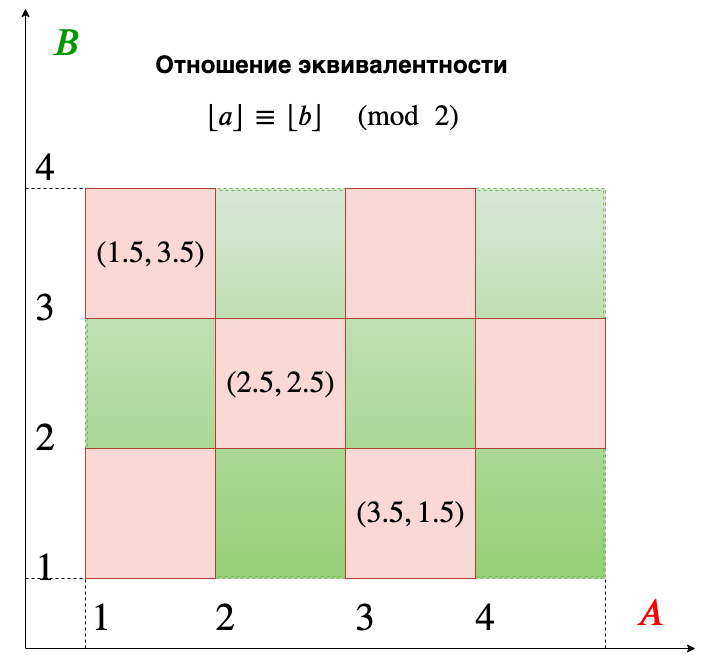
\includegraphics[scale=0.25]{equiv.png}
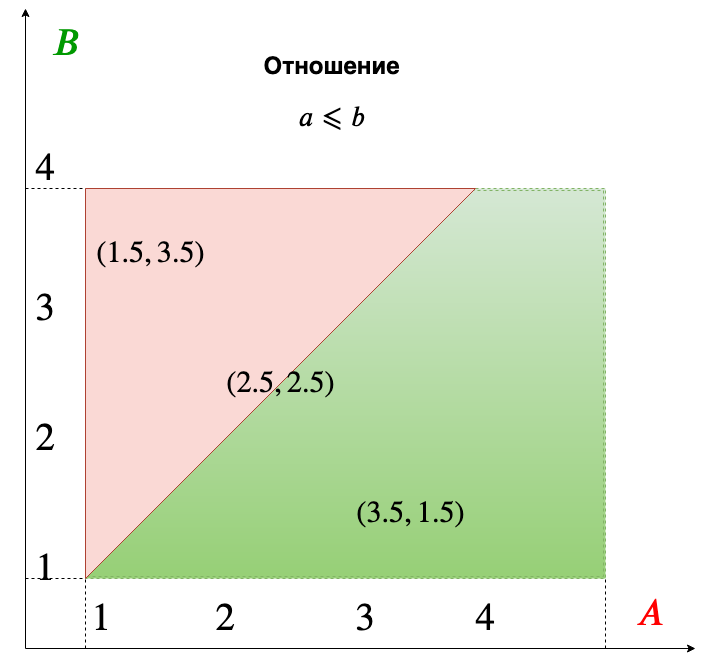
\includegraphics[scale=0.25]{lessthan.png}
\end{center}





\chapter{Движения плоскости и пространства}

\vrezka{Данная глава продолжает тему групп движений. Здесь мы получаем теорему Шаля (для движений плоскости), а затем широкими мазками освещаем тему движений сферы и пространства. 

Разделы о сфере и пространстве могут быть пропущены при первом ознакомлении с конспектом.
}

\section{Виды движений плоскости. Теорема Шаля}

\subsection*{Конспект}
\begin{enumerate}\setlength{\itemsep}{1pt}
\item Разбираем движения, попутно доказывая лемму <<о гвоздях>>.
\item Пусть на плоскости три точки, не лежащие на одной прямой, остаются неподвижными при движении. Вывод: это $\id$.
\item Пусть на плоскости неподвижны 2 точки и вся прямая, проходящая через них, остальные точки подвижны. Тогда это симметрия относительно данной прямой.
\item Пусть неподвижна лишь одна точка. Такое возможно лишь при вращении вокруг этой точки на угол, не кратный полному обороту.
\item Пусть вообще нет неподвижных точек. Берем любую точку, смотрим, куда она переходит, применяем сдвиг (параллельный перенос). Оставшееся преобразование имеет как минимум 1 неподвижную точку, а значит, является либо $\id$, либо симметрией, либо поворотом. Интересно, что поворот в данном случае можно исключить, т.к. композиция сдвига и поворота есть просто поворот, а значит, в исходном преобразовании была как минимум одна неподвижная точка. Следовательно, исходное движение есть либо сдвиг, либо смещенная симметрия (композиция сдвига и симметрии).
\item Таким образом, движение плоскости можно рассматривать как комбинацию параллельного переноса (в частности, на нулевой вектор), поворота (в частности, на нулевой угол) и симметрии относительно произвольной прямой.
\item \textbf{Теорема Шаля}. Произвольное движение (без разложения его на компоненты) есть движение одного из следующих классов:
\begin{enumerate}[a)]
\item класс параллельных переносов (на произвольный вектор), который мы обозначим $\rightrightarrows$;
\item класс поворотов относительно произвольного центра, который мы обозначим $\circlearrowleft$;
\item класс \textbf{скользящих симметрий} (сдвиг на произвольный вектор с последующей симметрией относительно оси данного вектора), который мы обозначим $\leftharpoonup\leftharpoondown$.
\end{enumerate}
\item Таблица композиций для таких классов выглядит следующим образом:
\begin{center}
\begin{tabular}{c|ccc}
 & $\rightrightarrows$ & $\circlearrowleft$ &  $\leftharpoonup\leftharpoondown$ \\ \hline
$\rightrightarrows$ & $\rightrightarrows$ &  $\circlearrowleft$ &  $\leftharpoonup\leftharpoondown$  \\ 
$\circlearrowleft$ & $\circlearrowleft$ & $\rightrightarrows$ или $\circlearrowleft$ & $\leftharpoonup\leftharpoondown$  \\ 
$\leftharpoonup\leftharpoondown$ & $\leftharpoonup\leftharpoondown$ & $\leftharpoonup\leftharpoondown$ & $\rightrightarrows$ или $\circlearrowleft$  \\ 
\end{tabular}
\end{center}
\item Аналогично одномерным случаям (прямая и окружность) можно выбирать различные базовые преобразования для построения с их помощью всех движений. 
\item Всякое движение есть композиция не более трех симметрий (относительно разных и, вообще говоря, не обязательно параллельных осей).
\item Сдвиг можно представить как композицию двух симметрий (относительно параллельных осей).
\item Поворот можно представить как композицию двух симметрий (относительно пересекающихся осей).
\item Скользящую симметрию можно представить как композицию трех симметрий (две на сдвиг и одна собственно симметрия).
\end{enumerate}


\subsection*{Задачи}
\begin{enumerate}
\item Показать, что композиция поворотов (относительно разных центров) есть либо сдвиг, либо поворот (вычислить его центр).
\item Показать, что композиция сдвига и поворота есть поворот.
\end{enumerate}


\section{Сравнение движений прямой, окружности и плоскости}
\subsection*{Конспект}
\begin{enumerate}
\item Отметим несколько общих свойств рассмотренных нами движений прямой, окружности и плоскости.
\item Во-первых, их всех можно свести к композиции симметрий. Для одномерных объектов (прямая и окружность) --- не более двух, для двумерных --- не более трех.
\item Во-вторых, все движения можно разделить на два класса: сохраняющие и меняющие \textbf{ориентацию}. Те движения, которые сводятся к композиции четного числа симметрий, сохраняют ориентацию фигур, а те, которые сводятся к композиции нечетного числа симметрий, --- меняют ориентацию фигур. Изменение ориентации означает, что право и лево меняются местами, т.е. мы как бы переходим в зазеркалье. 
\item При этом нужно отметить, что преобразования, меняющие ориентацию, обязательно требуют выхода в пространство, если мы хотим осуществить их непрерывным движением.
\item В-третьих, есть и более глубинная связь движений прямой, окружности и плоскости. Мы уже отмечали, что окружность можно рассматривать как прямую, у которой склеили противоположные концы (где-то на бесконечности). И с этой точки зрения сдвиг на прямой является прямой аналогией вращения окружности. Особенно, если величина сдвига сильно меньше радиуса.
\item А симметрия прямой при этом естественным образом превращается в симметрию окружности. Только ось симметрии должна проходить через место склейки двух бесконечностей. Остальные же симметрии можно получить дополнительным сдвигом, т.е. вращением.
\item Далее, окружность находится на плоскости. И поэтому вращение окружности полностью аналогично вращению плоскости, если при этом совместить их центры.
\item Еще проще увидеть совпадения понятий сдвига на прямой и плоскости. В обоих случаях мы просто смещаем все точки на какой-то вектор.
\item Тем не менее, на плоскости появляется новый вид движения, который комбинирует в себе сдвиг и отражение относительно оси сдвига. Это --- скользаящая симметрия, т.е. симметрия с последующим применением сдвига вдоль оси симметрии. На одномерных объектах такое движение в принципе невозможно. На прямой симметрия относительно этой же прямой ничего не дает, т.е. является $\id$, а на окружности симметрия относительно самой окружности вообще требует специального построения в геометрии плоскости.
\end{enumerate}


\section{Векторно-числовое представление движений плоскости}

\subsection*{Конспект}

\begin{enumerate}
\item \textbf{Аффинное пространство} --- множество точек и векторов. В аффинном пространстве мы работаем сразу с двумя сортами объектов --- точками и векторами, на которых заданы операции сложения и вычитания. При этом в сумме $a+b$ и разности $a-b$ могут быть такие комбинации:
\begin{enumerate}[1)]
\item $a$ --- точка, $b$ --- вектор, результатом $a+b$ будет точка, соответствующая концу вектора $b$, когда он отложен от точки $a$, результатом $a-b$ будет точка $c$ такая, что $c+b=a$;
\item $a$ и $b$ --- векторы, результатом $a+b$ будет вектор, построенный по правилу параллелограмма, результатом $a-b$ будет вектор $c$ такой, что $c+b=a$;
\item $a$ и $b$ --- точки, результатом $a-b$ будет вектор с началом в точке $b$ и концом в точке $a$.
\end{enumerate}
\item Движения --- это преобразования точек. Параметром движения может быть вектор и/или угол (число).
\item Сдвиг на плоскости на вектор $a$ обозначим $T_a$. Операция $T_a$ осуществляет прибавление вектора $a$ к точкам плоскости. Композиция сдвигов соответствует сумме векторов сдвига: $T_a\circ T_b=T_{b+a}$.
\item Поворот вокруг нуля мы ранее обозначали $R_\al$, где $\al$ --- угол в радианах.
\item Поворот на угол $\al$ относительно произвольной точки $M$ можно выразить так:
$$
R_{M,\al} = T_{O+M}\circ R_\al\circ T_{O-M},
$$
т.е. сначала сдвигаем точку $M$ в центр вращения, отмеченный точкой $O$, затем производим вращение, затем возвращаем точку $M$ на место обратным сдвигом.
\item Наконец, у нас остается такой вид движения, который осуществляет отражение относительно произвольной прямой на плоскости. Обозначим его $S_l$.
\item Предположим, что на плоскости помимо точки $O$ мы также зафиксировали некоторую прямую, проходящую через $O$ с выделенным направлением $OA$ ($A$ лежит на этой прямой и не совпадает с $O$). Зафиксируем отражение $S_{OA}$ относительно данной выбранной оси $OA$. Отметим, что $S_{OA}=S_{AO}$, т.е. отражение не зависит от направления оси отражения.
\item Выразим произвольное отражение через базовое отражение $S_{OA}$ и другие движения. Для этого обозначим через $M$  произвольную точку прямой $l$, через $\al$ --- угол наклона прямой $l$ относительно направления $OA$. Тогда
$$
S_l = T_{O+M}\circ R_\al \circ S_{OA} \circ R_{-\al}\circ T_{O-M},
$$
т.е. сначала мы сдвигаем плоскость так, чтобы точка $M$ оказалась в точке $O$, затем выполняем поворот на угол $-\al$, далее выполняем стандартное отражение, а затем производим обратные операции, которые возвращают прямую $l$ на место.
\item Соответственно, скользящая симметрия, при которой выполняется отражение относительно оси $l$ и сдвиг на вектор $MM'$ ($M,M'\in l$), записывается так:
$$
S_l = T_{O+M}\circ R_\al \circ S_{OA} \circ R_{-\al}\circ T_{O-M}\circ T_{M'-M},
$$
\item В терминах движений $T,R,S$ можно записать все возможные виды движений плоскости, т.е. сдвиг на произвольный вектор, поворот на произвольный угол относительно произвоьлной точки, скользящую симметрию относительно произвольной прямой $l$ со сдвигом на произвольный вектор, лежащий на этой прямой.
\item Если мы вернемся на окружность, то нам потребуется исключить сдвиги, оставив только вращения и симметрии.
\end{enumerate}




\section{Пара слов о движениях сферы}
\subsection*{Конспект}
\begin{enumerate}
\item Имея опыт перехода от прямой к окружности, мы можем легко найти движения сферы, отправляясь от движений плоскости.
\item Представим себе сферу как плоскость, у которой бесконечно удаленный край был стянут в точку (метод <<хинкали>>).
\item Во что превращаются при этом движения плоскости?
\item Сдвиг, он же параллельный перенос, превращается в такое движение, при котором все точки движутся по параллельным траекториям. С точки зрения географии это есть движение вдоль широтных линий. Да, проходят они при этом разное расстояние! Из-за чего, кстати, и появляются силы Кориолиса, создающие океанические течения вроде Гольфстрима. Но собственные расстояния между точками сохраняются, и это, несомненно, движение.
\item Вращение, которое, как мы помним, на окружности соответствует сдвигу на прямой, в случае сферы в прямом смысле слова совпадает со сдвигом! Дело в том, что вращение сферы вокруг оси, --- это вращение вокруг полюса, при котором угол поворота измеряется меридианом. Но ведь то же самое движение около экватора есть то, что мы только что отнесли к сдвигам вдоль широтных линий.
\item Таким образом, сдвиг прямой и вращение окружности в случае сферы чудесным образом объединяются в один вид движений --- осевое вращение. И это делает движения сферы чуть проще, чем движения плоскости, где сдвиг можно представить лишь как композицию двух вращений.
\item Далее, симметрия плоскости относительно прямой естественным образом переходит в отражение сферы относительно центральной секущей плоскости или, иначе говоря, относительно окружности большого круга. При такой симметрии полюса сферы меняются местами (полюса определются пересечением со сферой прямой, пересекающей плоскость отражения в центре сферы и перпендикулярной ей), а плоскость отражения остается на месте.
\item Наконец, скользящая симметрия плоскости есть композиция сдвига и осевой симметрии, и ей на сфере соответствует \textbf{зеркальное вращение}, т.е. композиция отражения и вращения параллельно плоскости отражения.
\item Таким образом, все движения сферы распадаются на два класса: вращения и зеркальные вращения. При этом, все движения есть композиция не более чем трех отражений.
\item Этот аналог теоремы Шаля для сферы можно доказать, используя очередную лемму о гвоздях, предполагая неподвижность пары противоположых точек (случай одной точки на плоскости), неподвижность целой окружности большого круга (случай двух точек на плоскости), отсутствие неподвижных точек.
\end{enumerate}

\subsection*{Задачи}
\begin{enumerate}
\item Построить таблицу движений сферы аналогично таблице движений плоскости (символику придумайте сами).
\item **Доказать, что других движений на сфере не существует (лемма о гвоздях).
\end{enumerate}


\section{Пара слов о движениях пространства}
\subsection*{Конспект}
\begin{enumerate}
\item Наконец, мы можем от сферы перейти к пространству. На самом деле, переход в пространство сопровождается лишь добавлением сдвига в пространстве. Т.е. любое движение сферы можно рассматривать как движение пространства с одной неподвижной точкой --- центром сферы. После чего можно применить сдвиг этого центра, и получить новые движения. Понятно, что никаких других движений тут быть не может.
\item Тем не менее, классификация движений пространства становится сложнее примерно так же, как классификация движений плоскости превосходит классификацию движений окружности. А именно, в пространстве появляется \textbf{винтовое движение} как композиция осевого вращения и сдвига вдоль оси вращения. Это --- обобщение скользящей симметрии на плоскости (если винт осуществляет поворот на $180^0$, мы как раз получаем скользящую симметрию).
\item Есть также и собственно \textbf{скользящая симметрия пространства}. Это --- отражение относительно плоскости с последующим сдвигом вдоль направления, параллельного данной плоскости. Такое движение также является обобщением скользящей симметрии на плоскости.
\item Заметим, что более сложное движение винт включает в себя более простые. Так, если винт имеет нулевой сдвиг, то он доставляет осевое вращение, а если винт имеет нулевой поворот, то он доставляет сдвиг. Понятно, что в случае полного зануления параметров винта мы получим $\id$.
\item Точно так же, \textbf{зеркальное вращение}, как и в случае сферы, при нулевом повороте доставляет просто симметрию.
\item Наконец, скользящая симметрия своим частным случаем имеет просто симметрию относительно плоскости.
\item Таким образом, классификация движений пространства включает следующие виды движений:
\begin{enumerate}[a)]
\item винт (в частности, сдвиг, осевое вращение, $\id$);
\item зеркальное вращение (в частности, отражение);
\item скользящая симметрия (в частности, отражение).
\end{enumerate}
\end{enumerate}

\subsection*{Задачи}
\begin{enumerate}
\item Построить таблицу движений пространства аналогично таблице движений плоскости (символику придумайте сами).
\item *Показать, что центральная симметрия пространства --- это зеркальное вращение.
\item **Доказать, что других движений в пространстве не существует (лемма о гвоздях).
\end{enumerate}


\begin{sidewaystable}
\caption{Сравнение движений.}
\label{Transitions}
\begin{tabular}{p{2cm}|p{2.5cm}p{2.5cm}p{2.5cm}p{2cm}p{2.5cm}p{2.5cm}}
\rowcolor{darkred}
& \multicolumn{3}{P{8.5cm}}{\textcolor{white}{\bfseries Собственные движения\linebreak (не меняют ориентацию)}} & \multicolumn{3}{P{8cm}}{\textcolor{white}{\bfseries Несобственные движения\linebreak (меняют ориентацию)}} \\ 
& Перенос & Поворот & Смещение поворота & Симметрия & \multicolumn{2}{p{5cm}}{Смещенная симметрия} \\ \hline \hline
Прямая     & сдвиг на число & & & относи\-тель\-но точки & & \\  \hline
Окруж\-ность & \multicolumn{2}{p{5cm}}{\centerline{вращение}} & & осевая симметрия & & \\ \hline
Плос\-кость  & параллель\-ный перенос & относи\-тель\-но точки & & осевая симметрия & скользящая симметрия (перенос+ сим\-мет\-рия) & \\  \hline
Сфера & вращение вблизи экватора & вращение вблизи полюса & & отражение относительно плоскости & \multicolumn{2}{p{5cm}}{зеркальное вращение (вращение+симметрия)} \\ \hline
Прост\-ранство & параллель\-ный перенос & осевое вращение & винт (перенос + вращение) & отражение относительно плоскости & скользящая симметрия (перенос+ сим\-мет\-рия) & зеркальное вращение (вращение+ сим\-мет\-рия) \\ \hline \hline
\end{tabular}
\end{sidewaystable}








\chapter{Перестановки}

\vrezka{
В этой главе мы в основном изучаем конечные группы а примере перестановок. Кроме того, дается промежуотчная сводка по свойствам групп.
}


\section{*Теория множеств: функции}\label{functions}

\subsection*{Конспект}

\begin{enumerate}
\item Введем понятие функции. Пусть у нас имеется отношение $F$ между множествами $X$ и $Y$. Отношение $F$ называется
\begin{enumerate}[{\bf Func1}]
\item \textbf{всюду значимым}, если для каждого $y\in Y$ найдется $x\in X$ такое, что $xFy$;
\item \textbf{всюду определенным}, если для каждого $x\in X$ найдется $y\in Y$ такое, что $xFy$;
\item \textbf{однозначным}, если всякий раз из одновременного выполнения $xFy$ и $xFy'$ следует, что $y=y'$, т.е. каждому $x$ соответствует не более одного $y$;
\item \textbf{обратно однозначным}, если всякий раз из одновременного выполнения $xFy$ и $x'Fy$ следует, что $x=x'$, т.е. каждому $y$ соответствует не более одного $x$;
\item \textbf{функцией из $X$ в $Y$}, если оно всюду определенное и однозначное;
\item \textbf{частичной функцией из $X$ в $Y$}, если оно однозначное;
\item (частичной) \textbf{сюръекцией из $X$ на $Y$}, если это всюду значимая (частичная) функция;
\item (частичной) \textbf{инъекцией из $X$ в $Y$}, если это обратно однозначная (частичная) функция;
\item \textbf{биекцией множеств $X$ и $Y$}, если это инъекция и сюръекция одновременно, т.е. отношение $F$ в данном случае взаимно однозначно связывает пары $(x,y)$.
\end{enumerate}
\begin{center}
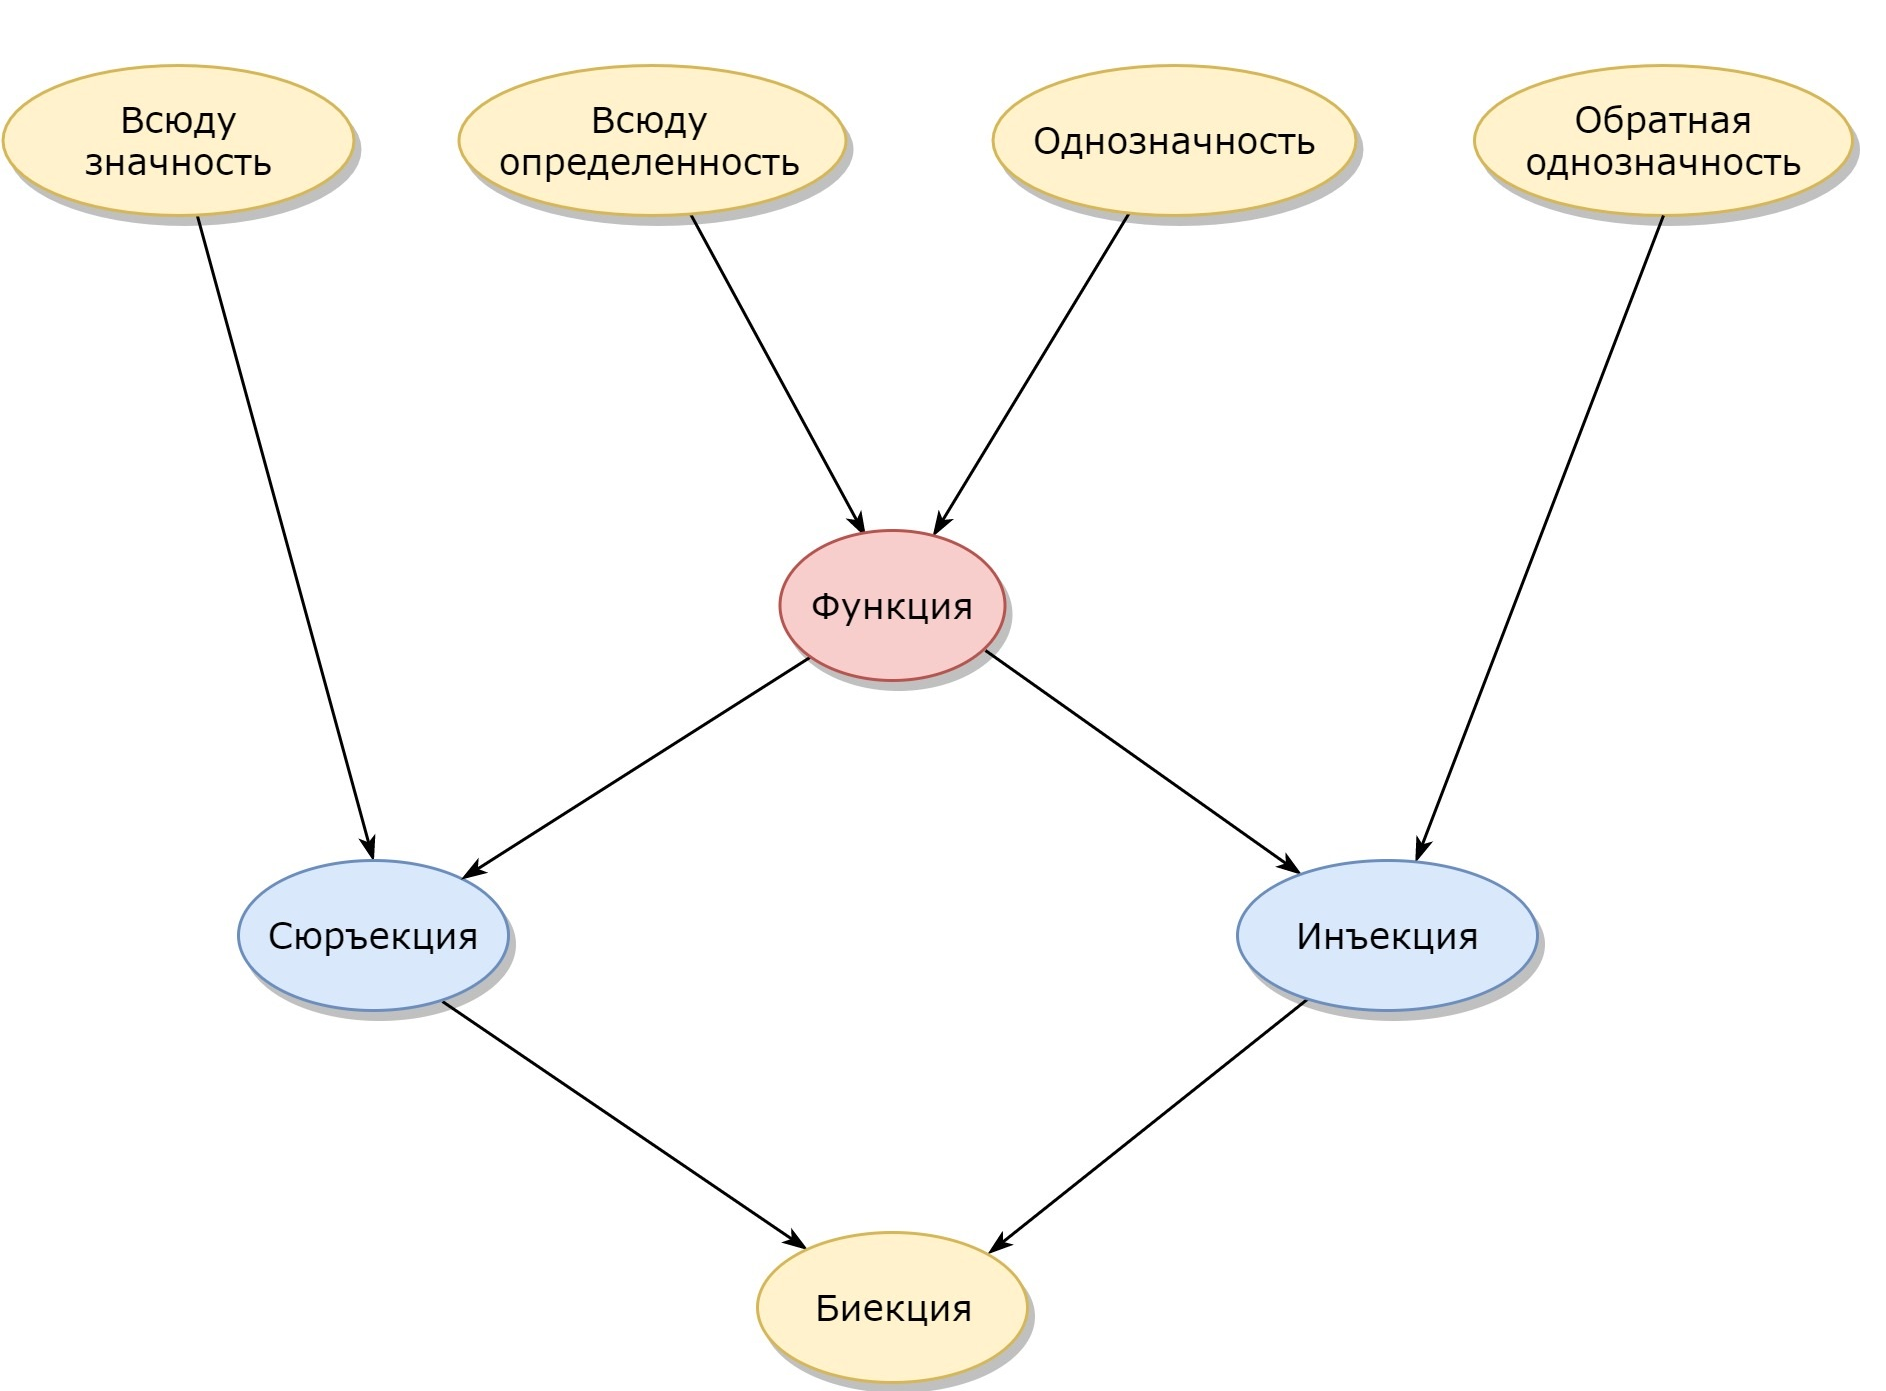
\includegraphics[scale=0.3]{function.png}
\end{center}

Обычно функция из $X$ в $Y$ обозначается $F:X\to Y$, а если $xFy$, то пишут $y=F(x)$. Для обозначения биекции часто используется символ $F:X\leftrightarrow Y$.
\item Обратным к $F$ отношением называется отношение $F^{-1}=\{(y,x)\mid xFy\}$. Если обратное отношение есть (частичная) функция, то она называется \textbf{обратной функцией}. Легко видеть, что $F(F^{-1}(y))=y$ и $F^{-1}(F(x))=x$, если только $F(x)$ и $F^{-1}(y)$ определены.
\item \textbf{Областью определения} функции $F$ называется множество $X$, а областью \textbf{определения частичной функции} $F$ --- подмножество $X$, для элементов которого $F$ определена, \textbf{областью значений} (частичной) функции $F$ называется подмножество $Y$, для элементов которого $F$ определена.
\item Итак, функция --- это есть однозначное соответствие элементов одного множества элементам другого (или того же самого). Функции обычно задаются формулами, предписывающими некоторой алгоритм вычисления $y$ через $x$. Но иногда такие формулы не указаны явно или же их указать вовсе невозможно, хотя существование функции строго доказывается (такие теоремы называют теоремами существования).
\end{enumerate}

\section{Конечные группы}

\subsection*{Конспект}

\begin{enumerate}
\item Рассмотрим группу $G$, состоящую из $n$ элементов, с операцией $\cdot$ (которую часто будем пропускать для удобства). В терминах функций операция $\cdot$ есть функция из $G\times G$ в $G$:
$$
\cdot: G\times G\to G.
$$

Напомним аксиомы группы:
\begin{enumerate}[G1]
\item $ab\in G$ для всех $a,b\in G$ (группоид);
\item для любых $a,b,c\in G$ имеем тождество $(ab)c=a(bc)$ (ассоциативность);
\item существует элемент $\e\in G$ такой, что $a\e=\e a=a$ для всех $a\in G$ (единица);
\item для всякого $a\in G$ существует обратный элемент $a^{-1}\in G$ такой, что $aa^{-1}=a^{-1}a=\e$ (обратный элемент).
\end{enumerate}
Кроме того, группа называется абелевой (или коммутативной), если $ab=ba$ для всех $a,b\in G$. Количество элементов в группе называется ее порядком.
\item В группе существует только одна единица. Действительно, если их две $\e$ и $\e'$, то в силу их же свойств получим
$$
\e' = \e\e' = \e
$$
(при первом равенстве мы рассматривали $\e$ как единицу, а при втором $\e'$).
\item Обратный элемент для каждого $a\in G$ определен однозначно. Предположим, что для элемента $a$ нашлось два обратных элемента $b,c$, т.е. $ab=ba=\e$ и $ac=ca=\e$. Тогда
$$
b=b\e=b(ac)=(ba)c=\e c=c.
$$
\item Степень элемента $\underbrace{a\cdots a}_{k\mbox{ раз}}$ обозначается $a^k$, где $k\in\N$. Кроме того, по определению, $a^0=\e$.
\item Отрицательная степень элемента по определению: $a^{-k}=(a^{-1})^k$, $k\in\N$.
\item Операции над степенями:
$$
(a^k)(a^m)=a^{k+m},
$$
где $k,m\in Z$. Если $k$ и $m$ одного знака, то это очевидно, а если разного, то пусть $k>0$, $m<0$, тогда
$$
(a^k)(a^m) = \underbrace{a\cdots a}_{k\mbox{ раз}}\underbrace{a^{-1}\cdots a^{-1}}_{|m|\mbox{ раз}}.
$$
Пользуясь ассоциативностью, начинаем сворачивать пары $aa^{-1}$, стоящие в середине, заменяя их на $\e$, а затем выбрасывая $\e$. В итоге либо ничего не останется (когда $k=-m$), либо останутся только $a$ в количестве $k+m$ (если $k>-m$), либо останутся только $a^{-1}$ в количестве $-m-k$ (когда $k<-m$). В любом случае это записывается как $a^{k+m}$ ($(a^{-1})^{-m-k}=a^{m+k}$ по определению).

\item В конечной группе каждый элемент в некоторой конечной степени обращается в $\e$. Действительно, все степени $a^k$ лежат в конечном множестве $G$, а число $k$ пробегает бесконечный науральный ряд. Следовательно, хотя бы два разных $k$ дадут один и тот же элемент (принцип Дирихле): $a^k=a^{k'}$, где $k<k'$. Домножим это равенство на $a^{-k}$ и получим $a^{k'-k}=\e$. Наименьший положительный показатель степени $m$ для элемента $a$, дающий равенство $a^m=\e$, называется порядком элемента $a$ в группе $G$.

Таким образом, в конечной группе у всякого элемента конечный порядок.

\item Отсюда следует, что всякую отрицательную степень элемента в конечной группе можно записать как положительную, поскольку
$$
a^k = a^{k\pmod p},
$$
где $p$ --- порядок элемента $a$.

\item Подмножество $T\subseteq G$, все возможные произведения степеней элементов которого, т.е. выражения вида $t_1^{k_1}\cdots t_m^{k_m}$, где $t_j\in T, k_j\in\N$ , образуют всю группу $G$, называется \textbf{системой образующих}\index{Группа!система образующих} группы $G$. При этом пишут $G=\langle T\rangle$ или $G=\langle t_1,\dots,t_m\rangle$.
\item Наименьшая по вложению система образующих группы называется \textbf{базисом}. Если базис состоит из одного элемента, тогруппа называется циклической. При этом ее можно записать так: $G=\langle g\rangle$, где $T=\{g\}$. Иначе говоря, циклическая группа состоит из степеней одного своего элемента.
\item Например, группа $\Z_n$ вычетов по модулю $n$ с операцией сложения является циклической: $\Z_n=\langle 1\rangle$, поскольку все ее элементы --- это конечные суммы единиц (от одной до $n$ штук). Группа вращений правильного $n$-угольника является циклической, где образующим элементом является поворот на угол $2\pi/n$. Группа $\Z_5^*$ с операцией умножения по модулю 5 является циклической вида $\langle 2\rangle$ и $\langle 3\rangle$.
\item Циклические группы являются абелевыми. Действительно, любые два элемента такой группы --- это некоторые степени образующего элемента, поэтому $(a^k)(a^m)=a^{k+m}=a^{m+k}=(a^m)(a^k)$. Коммутативность наследуется от группы $\Z$.

\item Подмножество $H\subseteq G$ называется подгруппой группы $G$, если $H$ само является группой с той же операцией, которая определена в $G$. Например, $\{0,2\}$ образует подгруппу группы $\Z_4$. Тривиальная подгруппа $\{\e\}$ является подгруппой любой группы.

\item Операции Минковского для подгруппы:
$$
gH=\{gh\mid h\in H\},\quad Hg=\{hg\mid h\in H\},
$$
где $gH$ называется левым, а $Hg$ --- правым классом смежности, порожденным элементом $g\in G$.

\item Классы смежности содержат одинаковое количество элементов.

Действительно, пусть $h_1\ne h_2$, где $h_1,h_2\in H$. Предположим, что $gh_1=gh_2$. Домножая слева на $g^{-1}$, находим, что $h_1=h_2$. Противоерчие. Следовательно, умножение на $g$ слева различные элементы переводит в различные. Аналогично --- для умнжения справа.

\item Классы смежности подгруппы $H$ либо совпадают, либо не пересекаются, а их объединение равно $G$. То есть, классы смежности образуют разбиение множества $G$. Такую ситуацию мы уже наблюдали в связи с подгруппами $m\Z$ и их сдвигами внутри $\Z$ и получали там $m$ классов смежности.

Пусть классы $g_1H$ и $g_2H$ имеют общий элемент $g$. Этот элемент будет иметь два представления: $g=g_1h_1=g_2h_2$, где $h_1,h_2\in H$, откуда $g_1=g_2h_2(h_1)^{-1}$. Возмем любой элемент $g_1h$ из первого класса, тогда
$$
g_1h = g_2h_2(h_1)^{-1}h,
$$
где $h_2(h_1)^{-1}h\in H$, т.к. $H$ --- подгруппа. Следовательно, $g_1h\in g_2H$, и $g_1H\subseteq g_2H$. Аналогично рассуждая, находим, что $g_2H\subseteq g_1H$, т.е. $g_1H=g_2H$.

Тот факт, что любой элемент $G$ находится в каком-то классе смежности, следует из того, что $\e\in H$, так что для любого $g\in G$ имеем $g\in gH$. И аналогично для правых классов.

\item Итак, множество $G$ есть сумма непересекающихся классов одного размера, причем размер классов равен порядку подгруппы $H$. Следовательно, порядок подгруппы делит подрядок группы. Это утверждение называется \textbf{теоремой Лагранжа}.\index{Теорема!Лагранжа о порядке группы}

\item $g_1H=g_2H$ тогда и только тогда, когда $(g_1)^{-1}g_2\in H$.

Пусть $g_1H=g_2H$, тогда любой элемент из этого множества имеет представление $g_1h_1=g_2h_2$, откуда $h_1(h_2)^{-1}=(g_1)^{-1}g_2$. Элемент слева --- это элемент подгруппы $H$.

Обратно, пусть $(g_1)^{-1}g_2=h\in H$, тогда $g_1h=g_2\e$. Элемент слева принадлежит $g_1H$, элемент справа --- $g_2H$, т.е. эти классы имеют общий элемент, а значит, совпадают.

\item Если группа имеет порядок $p$, где $p$ простое число, то такая группа является циклической.

Действительно, возьмем элемент $g\ne\e$ (поскольку $p>1$, то такое всегда возможно). Пусть $H=\langle g\rangle$ --- циклическая подгруппа $G$. Ее порядок делит порядок группы $G$, т.е. простое число $p$. В то же время, порядок $H$ отличен от 1, т.к. $H$ содержит как минимум два элемента $\e,g$. Но так как $p$ делится только на 1 и на $p$, то порядок группы $H$ равен $p$. Следовательно, $G=\langle g\rangle$.
\item Подгруппа $H$ группы $G$ называется \textbf{нормальной}\index{Группа!нормальная подгруппа}, если для любого $g\in G$ верно равенство $gH=Hg$, т.е. левые и правые классы не различаются. Обозначение: $H\vartriangleleft G$.

В абелевых группах любая подгруппа будет нормальной. В частности, $m\Z$ --- нормальная в $\Z$.
\item Классы смежности нормальной подгруппы можно умножать так же, как сами элементы группы $G$:
$$
(g_1H)(g_2H)=(g_1g_2)H.
$$
Это следует из того, что $(g_1h_1)(g_2h_2)=g_1(h_1g_2)h_2$, и при этом $h_1g_2=g_2h_3$ при некотором $h_3$ в силу нормальности $H$. Следовательно,
$$
(g_1h_1)(g_2h_2) = g_1(h_1g_2)h_2 = g_1(g_2h_3)h_2=(g_1g_2)(h_3h_2)\in (g_1g_2)H.
$$
Обратно, $(g_1g_2)h=(g_1\e)(g_2h)$. Здесь первый множитель принадлежит $g_1H$, второй $g_2H$. Так что мы имеем взаимное вложение множеств $(g_1H)(g_2H)$, $(g_1g_2)H$, т.е. их равенство.

\item Такое свойство умножения классов смежности по нормальной подгруппе позволяет задать групповую операцию на множестве всех классов смежности, которое обозначается
$$
G/H = \{gH\mid g\in G\}
$$
и называется \textbf{фактор-группой}\index{Группа!Фактор-группа} группы $G$ по нормальной подгруппе $H$. Опять же, мы уже всталкивались с примером фактор-группы $\Z/m\Z$ при изучении группы вычетов (см. раздел \ref{Faktor})

\item Факторизацию группы можно воспринимать как делимость групп, и в этом смысле группы становятся подобны числам. Есть простые группы --- они ни на что не делятся, а есть составные --- они делятся на нормальные подгруппы.

\item Естественно ввести и умножение групп. Пусть даны две группы $G_1$ и $G_2$ с операциями $\circ$ и $\star$, соответственно. Тогда на прямом произведении $G_1\times G_2$ определим операцию умножения по правилу
$$
(g_1,g_2)(g_1',g_2') = (g_1\circ g_1', g_2\star g_2'),
$$
т.е. будем покомпонентно перемножать все пары элементов прямого произведения. Легко проверить, что это --- групповая операция, т.е. она ассоциативна, имеет единицу, а для каждой пары есть обратная. Все эти свойства наследуются от исходных групп напрямую. Кроме того, если исходные группы абелевы, то и произведение групп будет абелевой группой. Такая конструкция называется внешним \textbf{прямым произведением групп} $G_1$ и $G_2$.

Если в исходных группах операция интерпретируется как сложение, то прямое произведение называют прямой суммой групп. Но, учитывая, что это может привести к путанице понятий, мы в любом случае будем пользоваться мультипликативной терминологией и символикой. Тем более, что она согласуется с теоретико-множественным прямым произведением.

\item Рассмотрим простой пример произведения групп: $\Z_2\times\Z_2$. Вот ее таблица умножения:

\begin{center}
\begin{tabular}{c|cccc}
$\Z_2\times\Z_2$ & 00 & 01 & 10 & 11\\  \hline
00 & 00 & 01 & 10 & 11 \\
01 & 01 & 00 & 11 & 10 \\
10 & 10 & 11 & 00 & 01 \\
11 & 11 & 10 & 01 & 00
\end{tabular}
\end{center}
где вместо пары $(i,j)$ мы про пишем $ij$ для краткости.

Видим, что эта группа абелева, но не циклическая. В этой группе есть три подгруппы $\{00,01\}$, $\{00,10\}$ и $\{00,11\}$.

Если сравнить ее с группой $\Z_4$ по сложению, то мы увидим существенную разницу. Во-первых, в $\Z_4$ только одна подгруппа $\{0,2\}$, а во-вторых, $\Z_4$ является циклической группой.

Этот пример показывает нам, что порядок группы не определят однозначно ее структуру (как нам того бы хотелось, памятуя об основной теореме арифметики).

Однако, нам уже хорошо знакома группа, которая имеет такую же таблицу умножения, как и $\Z_2\times\Z_2$. Это все та же группа симметрий ромба, т.е. четверная группа Клейна. Чуть позже мы к ней вернемся.

\item Говорят, что функция $f:G_1\to G_2$ является \textbf{изоморфизмом} групп $(G_1,\circ)$ и $(G_2,\star)$, если $f$ осуществляет взаимно однозначное соответствие обеих групп $g_2=f(g_1)$ так, что и результат операций в первой группе переходит в результат операций во второй:
$$
f(g_1\circ g_1') = f(g_1)\star f(g_1').
$$

Например, если мы рассмотрим группы $G_1=\Z_2\times\Z_2$ и $G_2=\Z_8^*$, то следующее соответствие
$$
01\mapsto 1,\quad 01\mapsto 3,\quad 10\mapsto 5, \quad 11\mapsto 7
$$
будет изоморфизмом этих групп. Это видно из следующих таблиц:

\begin{center}
\begin{tabular}{c|cccc}
$\Z_8^*$ & 1 & 3 & \cellcolor{lightRed} 5 & 7 \\  \hline
1 & 1 & 3 & 5 & 7 \\
3 & 3 & 1 & 7 & 5\\
5 & 5 & 7 & 1 & 3\\
7 & 7 & \cellcolor{lightRed} 5 & 3 & 1
\end{tabular}
\qquad
\begin{tabular}{c|cccc}
$\Z_2\times\Z_2$ & 00 & 01 & \cellcolor{lightRed} 10 & 11\\  \hline
00 & 00 & 01 & 10 & 11 \\
01 & 01 & 00 & 11 & 10 \\
10 & 10 & 11 & 00 & 01 \\
11 & 11 & \cellcolor{lightRed} 10 & 01 & 00
\end{tabular}
\end{center}

\end{enumerate}





\section{Арифметика перестановок}

\subsection*{Конспект}

\begin{enumerate}
\item Рассмотрим множество $X_n=\{x_1,\dots,x_n\}$, состоящее из $n$ элементов. На этом множестве рассмотрим все возможные биекции множества $X_n$ в себя. Обозначим
$$
\Sb(X_n) = \{f\mid f:X_n\leftrightarrow X_n\},
$$
проще говоря, это множество всех возможных \textbf{перестановок} элементов множества $X_n$.
\item Для функций, заданных на множестве, естественной операцией является операция композиции, т.е. последовательное применение функций друг к другу. Обычно композиция функций записывается символом $\circ$ или пропускается как умножение. Мы будем пользоваться первым вариантом, так что:
$$
(f\circ g)(x) = f(g(x))
$$
по определению.
\item Итак, мы имеем множество биекций (перестановок) с операцией композиции. Свойства композиции биекций таковы:
\begin{enumerate}[1.]
\item композиция биекций есть снова биекция;
\item $f\circ (g\circ h) = (f\circ g)\circ h$, поскольку это последовательное вычисление $f(g(h(x)))$;
\item существует функция, которая ничего не меняет: $\id(x)=x$, она также является биекцией;
\item для всякой биекции существует обратная функция, которая также является биекцией: $f\circ f^{-1}=f^{-1}\circ f=\id$;
\end{enumerate}

Таким образом, множество $\Sb(X_n)$ (и вообще, для любого множества $X$) с операцией композиции является группой. И называется группой перестановок множества $X_n$.
\item Один простой пример такой группы перестановок мы уже встречали, когда рассматривали все возможные симметрии правильного треугольника. Именно в этом случае все перестановки вершин треугольника оказались движениями, и только они.
\item Сколько всего перестановок в группе $\Sb(X_n)$?

Для ответа на этот вопрос посмотрим, сколько существует вариантов перехода одних элементов в другие. Очевидно, что первый элемент может перейти в любой, в том числе в самого себя, так что для него существует $n$ вариантов. Второй элемент может перейти куда угодно, кроме того места, которое занял первый, так что для него существует $n-1$ вариант. Третьему остается $n-2$ варианта. И т.д. Последнему элементу остается выбор из одного оставшегося места. Таким образом, всего вариантов перестановок на $n$ элементах существует ровно
$$
n(n-1)(n-2)\dots 2\cdot 1=n!
$$
Иначе говоря, группа $\Sb(X_n)$ имеет порядок $n!$.

\item Группа перестановок на 3х элементах имеет порядок $3!=6$, что соответствует количеству симметрий правильного треугольника.
Однако уже для квадрата число перестановок равно $24$, в то время как число всех движений составляет всего лишь 8, а для ромба так и вовсе 4. Вообще, как мы помним, количество движений правильного $n$-угольника равно $2n$. С ростом $n$ это число становится во много раз меньше, чем $n!$ (а точнее, в $3\cdot 4\cdots (n-1)=(n-1)!/2$ раз).
\item Чтобы не заострять внимание на происхождении элементов множества $X_n$, обычно они обозначаются числами от $1$ до $n$, так что $X_n=\{1,2,\dots, n\}$, а соответствующая группа биекций --- $\Sb_n$. Легко видеть, что группы $\Sb_n$ и $\Sb(X_n)$ изоморфны, т.е. между ними существует биекция, сохраняющая операцию композиции. Поэтому в дальнейшем, говоря о группе перестановок, мы будем иметь ввиду $\Sb_n$, заданную на множестве чисел $1,\dots, n$.
\item Теория групп в XIX в. начиналась именно с изучения групп подстановок, и лишь позже понятие группы было обобщено Артуром Кэли. Он же сделал первый важный шаг на пути классификации групп.
\begin{thrm}[Кэли]
Любая конечная группа порядка $n$ изоморфна некоторой подгруппе $\Sb_n$.
\end{thrm}
Для доказательства достаточно заметить, что каждый элемент $g$ исходной группы $G$ порождает биекцию на $G$ по правилу $h\mapsto gh$ (<<правые>> биекции), а эти биекции образуют изоморфную $G$ подгруппу внутри группы биекций на $G$.
\item В группе $\Sb_n$, как и в любой другой, можно построить циклическую подгруппу, отправляясь от произвольно взятого элемента, т.\,е. биекции на $X_n$. Например, пусть $s\in\Sb_n$, тогда можно рассмотреть циклическую подгруппу $G(s)=\{s,s^2,s^3,\dots\}$, где под степенью понимается многократная композиция биекции $s$ с самою собой. Ясно, что эта подгруппа не может быть бесконечной, т.\,к. она входит в конечную группу, поэтому при некотором $k$ имеем $s^k=\id$.

\item Рассмотрим некоторую перестановку $s\in \Sb_n$. Ее можно записать в виде таблицы аргумент--значение:
$$
s=
\begin{pmatrix}
1 & 2 & \dots & n-1 & n \\
s_1 & s_2 & \dots & s_{n-1} & s_n
\end{pmatrix}
$$
т.\,е. $s(i)=s_i$. При этом $\{1,2,\dots,n\}=\{s_1,s_2,\dots,s_n\}$ в полном соответствии с определением равенства множеств.

\item Возьмем теперь элемент 1 и начнем <<раскручивать>> его так же, как мы <<раскручивали>> степени элемента в циклической группе:
$$
1\mapsto s(1)\mapsto s(s(1))\mapsto\dots\mapsto s^k(1)
$$
Мы получим то, что называется \textbf{орбитой} элемента 1 при действии группы $G(s)$ на множестве $X_n$. Действительно, все элементы данной цепочки составляют множество $G(s)1=\{g(1)|\;g\in G(s)\}$. Кроме того, если $s^k=\e$, то $s^k(1)=1$, и мы получаем \textbf{цикл}:
$$
(1\; s(1)\; s(s(1))\;\dots\; s^{k-1}(1))
$$
(единицу в конце мы не пишем, подразумевая, что последний элемент цикла переходит в первый).

\item Действие группы $G(s)$ на множестве $X_n$ позволяет разбить это множество на несколько попарно непересекающихся орбит или циклов. Отсюда мы получаем представление самой перестановки $s$ как набора независимых циклов. Поэтому перестановки принято записывать в виде последовательности циклов. Например, пусть
$$
s=
\begin{pmatrix}
1 & 2 & 3 & 4 & 5 \\
2 & 4 & 1 & 3 & 5
\end{pmatrix}
$$
В этой перестановке мы наблюдаем два цикла: $(1 2 4 3)$ и тривильный $(5)$. Тогда
$$
s=(1 2 4 3)(5),
$$
причем, тривиальные циклы принято пропускать в такой <<циклической>> записи, т.\,к. они однозначно восстанавливаются по всем остальным циклам и по параметру $n$ (в нашем случае $n=5$).
\item Рассмотрим более сложный пример:
$$
s=
\begin{pmatrix}
1 & 2 & 3 & 4 & 5 & 6 & 7 \\
2 & 4 & 3 & 1 & 7 & 5 & 6
\end{pmatrix}
=(1 2 4)(3)(5 7 6)=(1 2 4)(5 7 6)
$$

\item Предположим теперь, что у нас имеется три перестановки:
$$
s_1=
\begin{pmatrix}
1 & 2 & 4 \\
2 & 4 & 1
\end{pmatrix}
\quad s_2=
\begin{pmatrix}
5 & 6 & 7 \\
7 & 5 & 6
\end{pmatrix}
\quad s_3=\id
$$
Тогда исходная перестановка $s$ получается как последовательное применение этих новых перестановок:
$$
s=s_1s_2s_3,
$$
причем порядок перестановок в композиции неважен, т.\,к. две их них <<работают>> на разных орбитах, а третья тождественна и коммутирует с любой перестановкой.

\item Таким образом, каждую перестановку из $\Sb_n$ можно единственным образом (с точностью до порядка) представить как композицию циклов, и, таким образом, запись перестановки в виде набора ее циклов является не только удобным соглашением, но еще и функционально верной.

\item Наконец, введем такое понятие как \textbf{транспозиция}. Это --- микроцикл, состоящий из двух элементов, например, (12) или (59) и т.п. Транспозиция меняет местами два элемента $X_n$, а остальные оставляет на месте. Любой цикл длины $k$ можно представить как композицию $k-1$ транспозиции. Например,\label{transpose}
$$
(1234) = (14)(13)(12),
$$
причем, это представление неоднозначное, поскольку:
$$
(2341) = (21)(24)(23),
$$
тем не менее, любая перестановка (не только цикл) имеет \textit{инвариант} по разложению в транспозиции.
\begin{thrm}
Если перестановка $g\in\Sb_n$ имеет два представления транспозициями
$$
t_1\dots t_k=g=\tau_1\dots\tau_m,
$$
то $k\equiv m\mod 2$.
\end{thrm}
Иначе говоря, четность перестановки, определяемая количеством входящих в ее разложение транспозиций, не зависит от способа этого разложения. Величина $\sgn(g)=(-1)^k=(-1)^m$ называется \textbf{знаком перестановки} $g$.

\item Функция $\sgn$, определенная на элементах группы $\Sb_n$ и принимающая значения из множества $B=\{-1,1\}$, является гомоморфизмом групп $\Sb_n$ и $B$ (проверьте, что $(B,\cdot)$ есть группа по умножению, изоморфная $\Z_2$).

\item В связи с этим дадим общее определение: \textbf{гомоморфизмом групп} $(G,\cdot)$ и $(G',\circ)$ называется всякая функция $h:G\to G'$, сохраняющая групповую операцию, т.\,е. $$h(g_1\cdot g_2)=h(g_1)\circ h(g_2).$$

Изоморфизм --- частный случай гомоморфизма. Ядром гомоморфизма $h$ называется прообраз единицы:
$$
\Ker(h)\rightleftharpoons h^{-1}\{\e'\}\rightleftharpoons\{g\in G|\;h(g)=\e'\},
$$
где $\e'$ --- единица группы $G'$.

Гомоморфизм обладает слеюущими свойствами
\begin{enumerate}[1$^\circ$]
\item Ядро гомоморфизма есть нормальная подгруппа: $\Ker(h)\vartriangleleft G$.
\item Если $H\vartriangleleft G$, то существует гомоморфизм $h:G\to G/H$ такой, что $H=\Ker(h)$.
\item Фактор-группа $G/\Ker(h)$ изоморфна образу $hG$ в группе $G'$.
\end{enumerate}

\item Нетрудно видеть, что функция $\sgn$ на группе $\Sb_n$ действует как гомоморфизм в группу $B$, поэтому прообраз 1 в группе $\Sb_n$ относительно данного гомоморфизма, а именно, \textit{все четные перестановки} образуют нормальную подгруппу в группе подстановок $\Sb_n$. Эта нормальная подгруппа обозначается $A_n$ и называется \textbf{знакопеременной группой} порядка $n$. Следует не путать употребленное здесь слово <<порядок>> с порядком группы, означающем количество ее элементов, поскольку в $A_n$ находится ровно половина элементов группы $\Sb_n$, т.\,е. $n!/2$, что значительно больше $n$.

\item Четность перестановки является инвариантом на подгруппе $A_n$ (т.е. принимает одно и то же значение на всех ее элементах), а также на ее смежном классе в $\Sb_n$ (принимает другое постоянное значение). Поиск инвариантов является одним из мощных математических инструментов при поиске закономерностей и доказательстве невозможности некоторых объектов или действий.
\item С конца XIX века известна игра <<пятнадцать>>, суть которой в следующем. Имеем поле 4x4, в котором расставлены одинаковые по размеру фишки размером 1x1. Всего фишек 15, и они пронумерованы числами от 1 до 15. Одно место на поле пустое, что позволяет производить следующие простые манипуляции: занимать данное место фишкой с любого смежного места, т.\,е. передвигать ее на это место, освобождая соседнее.
При этом нельзя совершать никакие другие действия, например, вынимать фишки с поля и расставлять их произвольным образом.

В результате таких действий порядок номеров у фишек меняется, т.\,е. мы осуществляем перестановку из группы $\Sb_{15}$.

<<Фишка>> этой игры в том, что все разрешенные манипуляции не меняют четности исходной перестановки номеров. А это значит, что никакую нечетную изначальную расстановку невозможно привести (разрешенными действиями) к четной перестановке, и наоборот. Например, две расстановки фишек, отличающиеся лишь одной транспозицией (обменом двух соседних фишек местами), не могут быть переведены одна в другую.

Создатель игры (никто еще не знал тогда алгебраического решения задачи) даже обещал приз 100 долларов тому, кто приведет расстановку
\begin{center}
\begin{tabular}{|c|c|c|c|}
\hline
1 & 2 & 3 & 4 \\ \hline
5 & 6 & 7 & 8 \\ \hline
5 & 6 & 7 & 8 \\ \hline
9 & 10 & 11 & 12 \\ \hline
13 &15 & 14 & \\ \hline
\end{tabular}
\quad к виду \quad
\begin{tabular}{|c|c|c|c|}
\hline
1 & 2 & 3 & 4 \\ \hline
5 & 6 & 7 & 8 \\ \hline
5 & 6 & 7 & 8 \\ \hline
9 & 10 & 11 & 12 \\ \hline
13 &14 & 15 & \\ \hline
\end{tabular}
\end{center}
(они отличаются транспозицией (15\ 14)).

С тех пор прошло больше 100 лет, и до сих пор многие пытаются это сделать, но алгебра дает нам беспощадный ответ: это сделать невозможно! Потому что четность перестановки инвариантна относительно действий с фишками!

\item Другой замечательный пример инварианта --- теорема Эйлера о числе выпуклого многогранника: величина В-Р+Г=2 для всех выпуклых многогранников (В --- число вершин, Р --- ребер, Г --- граней). Отсюда, в частности, следует, что на футбольном мяче, сшитом только из правильных 5- и 6-угольников, может быть только 12 пятиугольников, никакое другое число не удовлетворяет этому инварианту.


\item Как уже отмечалось выше, все конечные группы изоморфны некоторым подгруппам в группах перестановок. Ранее изученная нами 
группа $\Z_2\times\Z_2$ имеет изоморфный клон среди подгрупп группы перестановок $\Sb_4$. В таблице \ref{SymmetricS4} (в конце книги) помещена полная таблица умножения группы $\Sb_4$ с использованием кратких обозначений перестановок как произведений циклов. Там же выделены две подтаблицы, отвечающие группам $A_4$ и $V_4$, а также отмечены (жёлтым) элементы (и их произведения) подгруппы 8-го порядка, которая не является ни нормальной, ни абелевой.

Выделенная подгруппа 8-го порядка:
$$\{\e, (12)(34), (13)(24), (14)(23), (12), (34), (1324), (1423)\}.
$$
Все подгруппы 8-го порядка изоморфны. Аналогичная ситуация с подгруппами 6-го порядка, вот одна из них:
$\{\e, (123), (132), (12), (13), (23) \}$, которая совпадает с $\Sb_3$.

\item В группе $\Sb_4$ существует только 2 нетривиальные нормальные подгруппы: $A_4$ и $V_4$. Все подгруппы порядков 2,3,6,8 не являются нормальными.

\item Говорят, что группа $G$ имеет \textbf{субнормальный ряд} (называемый также \textbf{субнормальной башней}, \textbf{субинвариантным рядом}, \textbf{субнормальной матрёшкой} или просто \textbf{рядом}) длины $n$, если имеют место вложения:
$$
\{\e\}=G_0\vartriangleleft G_1\vartriangleleft\dots\vartriangleleft G_{n-1}\vartriangleleft G_n=G,
$$
где $G_i$ --- собственная нормальная подгруппа в $G_{i+1}$. Ряд называется \textbf{нормальным}, если все $G_i$ нормальны также в исходной группе $G$. Факторгруппы $G_{i+1}/G_i$ называются \textbf{факторами} (факторгруппами) \textbf{ряда}.

Для простых групп (например, $\Z_p$) тривиальный субнормальный ряд длины 1 является единственно возможным: $\{\e\}\vartriangleleft G$.

Для группы $\Sb_4$ имеем: 
$$
\{\e\}\vartriangleleft V_4\vartriangleleft A_4\vartriangleleft\Sb_4,\quad\{\e\}\vartriangleleft V_4\vartriangleleft\Sb_4
$$
Эти утверждения можно извлечь непосредственно из таблицы \ref{SymmetricS4}. Например, нормальность $V_4$ в $A_4$ следует из того, что симметричные столбец и строка в зеленой области напротив и под группой $V_4$ совпадают с точностью до перестановки элементов (т.\,е. выполняется условие $gH=Hg$).

\item Если для группы $G$ существует такой субнормальный ряд, что все его факторы --- абелевы группы, то группа $G$ называется \textbf{разрешимой}.

Так как
\begin{enumerate}[a)]
\item $\Sb_4/A_4\simeq\Z_2$, т.\,е. является циклической и, тем более, абелевой группой,
\item $A_4/V_4\simeq\Z_3$, т.\,е. является циклической и, тем более, абелевой,
\item $V_4/\{\e\}$ --- абелева группа (см. таблицу \ref{SymmetricS4}),
\end{enumerate}
то $\Sb_4$ разрешима. Заметим, что ряд $\{\e\}\vartriangleleft V_4\vartriangleleft\Sb_4$ не годится для установления разрешимости, поскольку фактор $\Sb_4/V_4\simeq\Sb_3$ не является абелевой группой.

Для $n=3$ имеем $\{\e\}\vartriangleleft A_3\simeq\Z_3\vartriangleleft\Sb_3$ и, таким образом, $\Sb_3$ также разрешима. Тем более разрешима и $\Sb_2\simeq\Z_2$.

Известно, что все $\Sb_n$ порядка $n\ge 5$ неразрешимы. Именно на этом замечательном факте построено доказательство знаменитой теоремы Галуа о неразрешимости в радикалах уравнений степени 5 и выше.

\end{enumerate}





\section{Четверная группа Клейна}

\noindent
\begin{tabular}{c||c}
Четверная группа Клейна & Циклическая 4-го порядка \\ \hline\hline
\\

\begin{tabular}{c|cccc}
$\Diamond$ & $\id$     & $R$   & $S_1$ & $S_2$ \\ \hline
     $\id$ & $\id$     & $R$   & $S_1$ & $S_2$ \\ 
     $R$   & $R$       & $\id$ & $S_2$ & $S_1$ \\
     $S_1$ & $S_1$     & $S_2$ & $\id$ & $R$ \\
     $S_2$ & $S_2$     & $S_1$ & $R$   & $\id$
\end{tabular}
 & \footnotesize
\begin{tabular}{c|cccc}
$\Box$ & $\id$ & $R_{\pi/2}$ & $R_{\pi}$ & $R_{3\pi/2}$ \\[1pt]  \hline \\[-6pt]
$\id$  & $\id$ & $R_{\pi/2}$ & $R_{\pi}$ & $R_{3\pi/2}$ \\[3pt]
$R_{\pi/2}$  & $R_{\pi/2}$ & $R_{\pi}$ & $R_{3\pi/2}$ & $\id$ \\[3pt]
$R_{\pi}$ & $R_{\pi}$ & $R_{3\pi/2}$ & $\id$ & $R_{\pi/2}$\\[3pt]
$R_{3\pi/2}$ & $R_{3\pi/2}$ & $\id$ & $R_{\pi/2}$ & $R_{\pi}$
\end{tabular}
\\

\\


\begin{tabular}{c|cccc}
$\Z_8^*$ & 1 & 3 & 5 & 7 \\  \hline
1 & 1 & 3 & 5 & 7 \\
3 & 3 & 1 & 7 & 5\\
5 & 5 & 7 & 1 & 3\\
7 & 7 & 5 & 3 & 1
\end{tabular}
 &
\begin{tabular}{c|cccc}
$\Z_4$ & 0 & 1 & 2 & 3 \\  \hline
0 & 0 & 1 & 2 & 3 \\
1 & 1 & 2 & 3 & 0\\
2 & 2 & 3 & 0 & 1\\
3 & 0 & 1 & 2 & 3
\end{tabular}
\\

\\


\begin{tabular}{c|cccc}
$\Z_2\times\Z_2$ & 00 & 01 & 10 & 11\\  \hline
00 & 00 & 01 & 10 & 11 \\
01 & 01 & 00 & 11 & 10 \\
10 & 10 & 11 & 00 & 01 \\
11 & 11 & 10 & 01 & 00
\end{tabular}
 &
\begin{tabular}{c|cccc}
$\Z_5^*$ & 1 & 2 & 4 & 3 \\  \hline
1 & 1 & 2 & 4 & 3 \\
2 & 2 & 4 & 3 & 1\\
4 & 4 & 3 & 1 & 2\\
3 & 3 & 1 & 2 & 4
\end{tabular}
\\
\\

\footnotesize %\sffamily
\begin{tabular}{cc|cc}
 $\id$    & (12)(34) & (13)(24) & (14)(23) \\[5pt]
 (12)(34) & $\id$    & (14)(23) & (13)(24) \\[3pt]\hline
 &&& \\[-5pt]
 (13)(24) & (14)(23) & $\id$    & (12)(34) \\[5pt]
 (14)(23) & (13)(24) & (12)(34) & $\id$
\end{tabular}
 &
\begin{tabular}{c|cccc}
$\sqrt[4]{1}$ & 1    & $i$  & $-1$ & $-i$ \\  \hline
1             & 1    & $i$  & $-1$ & $-i$ \\
$i$           & $i$  & $-1$ & $-i$ & 1    \\
$-1$          & $-1$ & $-i$ & 1    & $i$  \\
$-i$          & $-i$ & 1    & $i$  & $-1$
\end{tabular}
\\
\\

\hline

\end{tabular}



\section{Перестановки: деликатесы}




\chapter{Линейные уравнения}

\vrezka{
Основная задача данной главы --- дать полное описание решений линейных уравнений в целях числах. Попутно вводится уравнение прямой на координатной плоскости, хотя мы все еще подразумеаем, что работаем только с целыми числами.
}

\section{Уравнение прямой на плоскости}

\subsection*{Конспект}

\begin{enumerate}
\item Рассмотрим плоскость с координатными осями $Ox$ и $Oy$. Что будет, если ее начать поворачивать? Во что переходит при этом ось $Ox$?
\item Поскольку вращение --- это движение, расстояние между точками сохраняется, и значит, никакие три точки, лежащие на прямой $Ox$, при повороте не могут перейти в точки, образующие невырожденный треугольник --- они снова лягут на прямую, причем в том же самом порядке. Стало быть, $Ox$ при вращении плоскости переходит в некоторую прямую.
\item Пусть центорм вращения является точка $O=(0,1)$, и ось $Ox$ при вращении $R_\ph$ переходит в прямую $l$. Ясно, что $l$ такаже проходит через начало координат $O$, т.к. это --- стационарная точка вращения.
\item Фиксируем на $Ox$ точку $(1,0)$ и посмотрим, куда она переходит под действием всех возможных вращений. Поскольку расстояние от центра вращения сохраняется, ясно, что эта точка остается на окружности радиуса 1. В то же время, выбирая произвольную точку на этой окружности, мы легко укажем угол $\ph$, на который нужно осуществить поворот плоскости относительно центра $O$, чтобы точка $(1,0)$ перешла в выбранную нами точку.
\item Итак, под действием группы вращений точка $(1,0)$ переходит во все точки единичной окружности. Аналогично, если мы выберем произвольную точку $(r,0)$ ($r>0$), она будет переходить во все точки окружности радиуса $r$ под действием группы вращений с центром в точке $O$.
\item В этом случае принято говорить, что группа вращений \textbf{действует} на плоскости, а множество всех значений, в которые она переводит выбранную точку, называют \textbf{орбитой} этой точки. В нашем примере орбитами являются коцентрические окружности с центром $O$.
\item Можно доказать, что орбиты образуют классы экивалентности, т.е. они попарно не пересекаются и в сумме дают всю область действия группы.
\item Фиксируем некоторое вращение $R_\ph$, и пусть точка $(0,1)$ при таком вращении перешла в точку $C=(x_0,y_0)$, лежащую на единичной окружности.
\item Возьмем произвольную точку $(r,0)$, где $r>0$, и проследим ее судьбу под действием того же вращения $R_\ph$. Пусть $A=(x,y)=R_\ph(r,0)$. Ясно, что точки $O,C,A$ лежат на одной прямой $l$.
\item Проведем вертикальные линии через абсциссы $x_0$ и $x$, а также горизонтальные линии через ординаты $y_0$ и $y$. Добавим новые точки пересечения $B$ и $D$ (см. рисунок).

\begin{center}
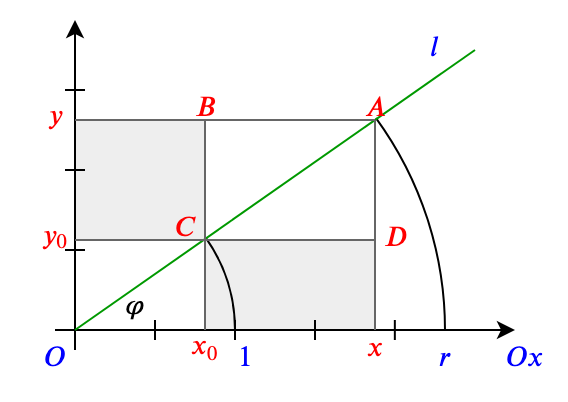
\includegraphics[scale=0.5]{linerotation.png}
\end{center}
\item Видим, что треугольники $ABC$ и $ADC$ равны по трем сторонам, также равны треугольники $Oy_0C$ и $Ox_0C$, и треугольники $OyA$ и $OxA$. Отсюда легко установить равенство площадей $x_0(y-y_0)=y_0(x-x_0)$, откуда получаем
$$
xy_0-yx_0=0.
$$
\item Поскольку $(x,y)$ --- это произвольная точка прямой $OC$ (для отрицательного $r$ все доказывается аналогично),  данное уравнение есть уравнение прямой, проходящей через начало координант с углом наклона $\ph$.
\item Отметим, что точка $(x_0,y_0)$ полностью определяется углом поворота $\ph$, т.к. является образом точки $(0,1)$ при повороте на угол $\ph$. В то же время, произвольная точка на единичной окружности однозначно задает угол поворота в интервале от 0 до $2\pi$. Таким образом, задать поворот с центром $O$ и задать точку на единичной окружности --- суть одно и то же.
\item Зная тригонометрию, можно также заметить, что $x_0=\cos\ph$ и $y_0=\sin\ph$, а отношение $y_0/x_0=\tan\ph$.
\item Кроме того, отношение $y_0/x_0$ также однозначно определяет угол поворота, но только в интервале от 0 до $\pi$.
\item Наконец, поворот прямой(!) на угол $\pi+\al$ --- это поворот на угол $\al$ с последующим отражением прямой $l$ относительно точки $O$. Но отражение прямой относительно своей же точки дает нам ту же самую прямую с тем же самым уравнением для ее точек! Таким образом, прямая, проходящая через начало координат полностью определяется тангенсом угла наклона, т.е. отношением $y_0/x_0$.
\item Но раз все дело в отношении, стало быть, прямая задается любой точкой, координаты которой находятся в таком же соотношении, что и коодинаты точки $(x_0,y_0)$, лежащие на единичной окружности. Иначе говоря, одну и ту же прямую задают также точки вида $(-x_0,-y_0)$, $(rx_0,ry_0)$, $(-rx_0,-ry_0)$, если коэффициент $r>0$. На рис. мы обозначили эти точки, соответственно, $C,A$ и $-C,-A$.
\begin{center}
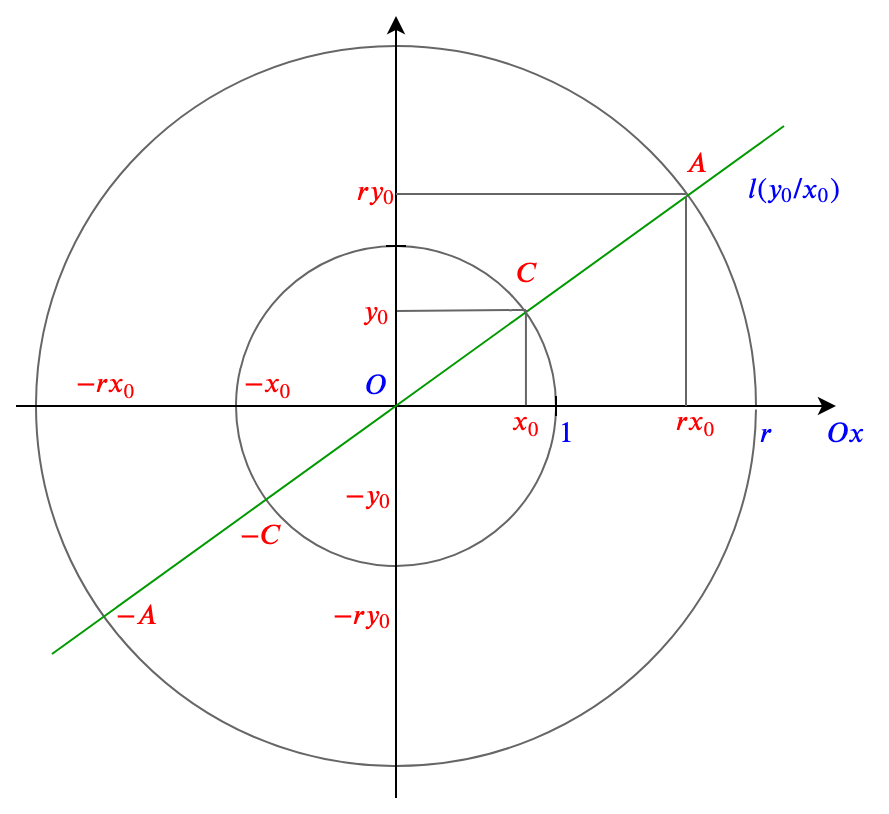
\includegraphics[scale=0.3]{line.png}
\end{center}
\item Этот вывод можно получить и более формально, просто глядя на уравнение прямой
$$
xy_0-yx_0=0.
$$
Ведь если мы домножим обе части уравнения на $r$, ничего не изменится!
$$
x(ry_0)-y(rx_0)=0.
$$
\item Что если прямая $l$ не проходит через центр координат $O$? В этом случае мы можем сдвинуть ее на некоторый вектор так, чтобы произвольно выбранная точка этой прямой перешла в точку $O$. Обозначим эту точку на прямой $l$ за $S=(\De x,\De y)$, а сдвиг, соответственно, осуществим на вектор $(-\De x,-\De y)$.
\begin{center}
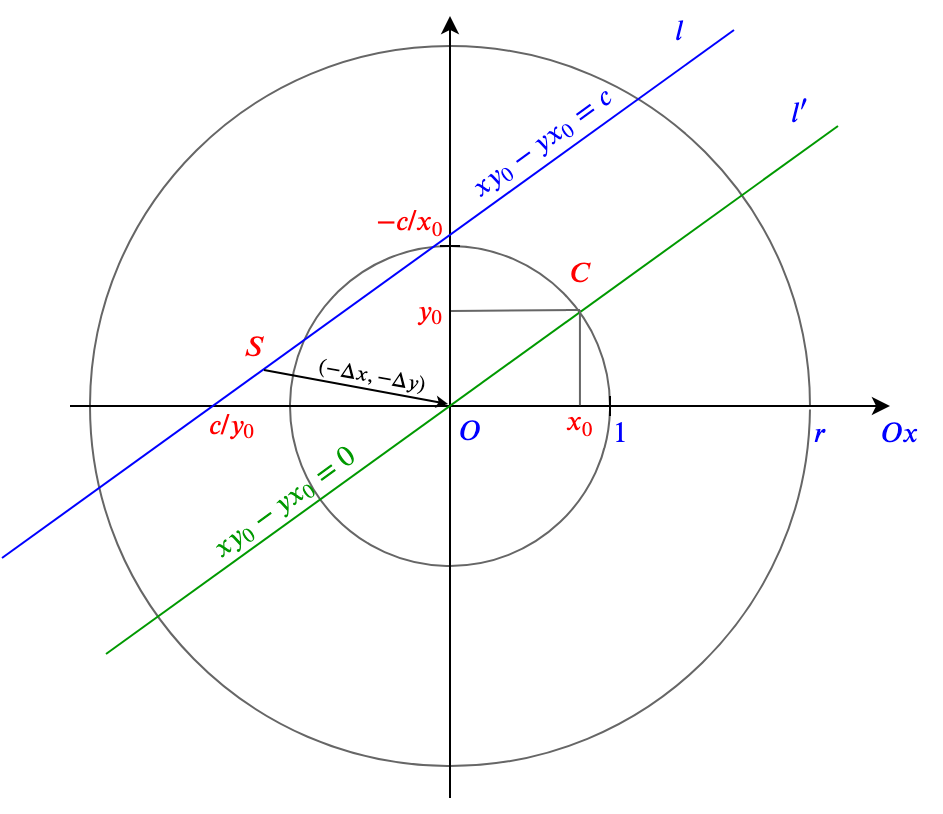
\includegraphics[scale=0.3]{lineshift.png}
\end{center}
\item Тогда смещенные координаты $(x-\De x,y-\De y)$ уже будут пробегать прямую $l'$, проходящую через центр $O$, а ее уравнение нам известно:
$$
(x-\De x)y_0 - (y-\De y)x_0=0,
$$
или
$$
xy_0-yx_0=c,\quad\mbox{где } c= y_0\De x - x_0\De y.
$$
При этом коэффициенты $(x_0,y_0)$ все так же отвечают за наклон прямой $l$ и полностью определяются тангенсом угла наклона прямой $l$ относительно положительного направления $Ox$, т.е. отношением $y_0/x_0$.
\item Может показаться, что уравнение сильно зависит от выбора точки $S$, поскольку слагаемое $c$ зависит от координат точки $S$. Покажем, что это не так. Пусть $S'=(\De x',\De y')$ --- какая-то другая точка прямой $l$. Но в этом случае она удовлетворяет найденному уравнению, т.е.
$$
\De x'y_0-\De y'x_0=c,
$$
но уравнение, найденное с помощью точки $S'$ будет иметь вид
$$
xy_0-yx_0= y_0\De x' - x_0\De y',
$$
откуда из предыдущего получаем, что вновь
$$
xy_0-yx_0=c.
$$
\item Таким образом, для нахождения $c$ мы можем выбрать любую понравившуюся нам точку прямой $l'$, например, отчку пересечения с одной из координатных осей.
\item В случае, когда $x_0\ne 0$, уравнение прямой можно переписать в виде
$$
y  = ax+b,\quad\mbox{где }a=\frac{y_0}{x_0},\; b=-\frac{c}{x_0}.
$$
В случае $x_0=0$ мы имеем вертикальную прямую $x=c$ (при угле $\ph=\pi/2$ мы получим $y_0=1$).
\end{enumerate}
\subsection*{Задачи}

\begin{enumerate}
\item В какие точки переходят точки $(0,3)$ и $(4,0)$ при повороте на $90$ градусов? На $-90$ градусов?
\item Каков угол поворота, если точка $(a,b)$ перешла в точку $(-a,-b)$? В точку $(-b,a)$? В точку $(b,-a)$?
\item Чему равен тангенс угла наклона прямой $3x-5y=7$?
\item Какой угол наклона у прямой $y=-x+3$?
\end{enumerate}


\section{Линейные уравнения в целых числах}

\subsection*{Конспект}

\begin{enumerate}
\item Поскольку мы пока владеем аппаратом только целых чисел (множество $\Z$), рассмотрим задачу о нахождении всех целых точек плоскости, через которые проходит заданная прямая. Под целыми точками плоскости мы будем понимать такие точки, координаты которых принадлежат $\Z$.
\item В общем виде \textbf{линейное уравнение в целых числах} выглядит следующим образом:
$$
ax-by=c,\quad\mbox{где коэффициенты } a,b,c\in\Z.
$$
Задача: найти все такие $x,y$, тоже целые, которые удовлетворяют данному уравнению.
\item Сначала рассмотрим случай т.н. \textbf{однородного уравнения}:
$$
ax-by=0,
$$
т.е. мы отбрасываем ту часть уравнения, которая не зависит от переменных $x,y$.
\item Как мы уже знаем, данное уравнение задает прямую, проходящую через начало координат, а ее наклон определяется отношением $a/b$.
\item Для начала проверим, нельзя ли данное отношение упростить. Если числа $a,b$ имеют какой-то общий делитель, то разумно было бы на него сократить. И чтобы не проверять это много раз, сократим их сразу на $\gcd(a,b)$. Множество решений от этого не изменится, а само уравнение по-прежнему останется однородным и целочисленным:
$$
\tilde ax-\tilde by=0,\quad\mbox{где } \tilde a=\frac{a}{\gcd(a,b)},\;\tilde b=\frac{b}{\gcd(a,b)}.
$$
\item Таким образом, мы приходим к уравнению со взаимно простыми коэффициентами $\tilde a$ и $\tilde b$.
\item Перепишем уравнение иначе: $\tilde ax=\tilde by$. Заметим, что все числа здесь --- целые. Причем $\tilde by$ делится на $\tilde a$. Но так как $\tilde a$ и $\tilde b$ взаимно просты, то $y$ делится на $\tilde a$. Это есть следствие того факта, который мы доказывали ранее в разделе \ref{PrimeNumbers}: если простое число $p$ делит произведение $ab$, то оно делит $a$ или $b$ (или их обоих). Поэтому если простое $p$ делит $\tilde a$, то оно делит $\tilde by$, но оно не может делить $\tilde b$, т.к. $\gcd(p,\tilde b)=1$, значит, оно делит $y$. Это значит, что все простые, составляющие число $\tilde a$, являются делителями $y$. В то же время, эти простые не входят в $\tilde b$, поскольку $\gcd(\tilde a,\tilde b)=1$. Поэтому, если $p^\al$ входит в разложение $\tilde a$, то $p^\al$ также делит $y$. Следовательно, $y$ делится на $\tilde a$, т.е. 
$$
y=k\tilde a
$$
при некотором целом $k$.
\item Симметрично рассуждая, получаем, что $x$ делится на $\tilde b$, т.е.
$$
x=t\tilde b
$$
при некотором целом $t$.
\item Подставим эти выражения в наше однородное уравнение:
$$
\tilde a(t\tilde b)=\tilde b(k\tilde a),
$$
откуда
$$
t=k,
$$
и больше никаких ограничений на выбор коэффициента $k$ мы не имеем.
\item Таким образом, решениями уравнения $\tilde ax-\tilde by=0$ являются
$$
\begin{cases}
x  =k\tilde b=kb/\gcd(a,b), \\
y  =k\tilde a=ka/\gcd(a,b),
\end{cases}
$$
где $k\in\Z$. Эти же $x$ и $y$ являются решениями исходного однородного уравнения $ax-by=0$.
\item Вернемся к неоднородному уравнению $ax-by=c$.
\item Для начала заметим, что если данное уравнение имеет решение в целых числах, то $ax-by$ делится на $\gcd(a,b)$, а значит, $c$ делится на $\gcd(a,b)$. Поэтому, если $c$ не делится на $\gcd(a,b)$, то решений точно нет, т.е. в таком случае прямая $ax-by=c$ проходит мимо всех целых точек плоскости!
\item Покажем, что в случае делимости $c$ на $\gcd(a,b)$ решения обязательно есть, и опишем все такие решения.
\item Пусть $c=d\gcd(a,b)$.
\item В разделе \ref{PrimeNumbers} мы установили, что $\gcd(a,b)$ является линейной комбинацией чисел $a$ и $b$, т.е.
$$
\gcd(a,b) = an-bm
$$
при некоторых целых $n$ и $m$ (понятно, что знак перед $m$ можно выбирать любой, поэтому выберем так, как нам удобнее).
\item Отсюда следует, что пара чисел $(dn,dm)$ удовлетворяет уравнению $ax-by=c$, поскольку
$adn-bdm=d\gcd(a,b)=c$.
\item Итак, представив $\gcd(a,b)$ в виде линейной комбинации $a$ и $b$, мы можем найти одно решение исходного уравнения.
\item Далее применим тот же прием, что и при изучении уравнений прямых --- сдвинем прямую $ax-by=c$ так, чтобы точка $(dn,dm)$ оказалась в начале координат. Для этого введем новые переменные
$$
\hat x = x-dn,\quad \hat y = y-dm.
$$
\item Тогда получаем, что $a\hat x-b\hat y = 0$. А такое уравнение мы уже решили выше, и его решением будет пара чисел $\hat x = kb/\gcd(a,b)$ и $\hat y = ka/\gcd(a,b)$, где $k$ --- любое целое число.
\item Собирая все вместе, находим общее решение исходного уравнения:
$$
\begin{cases}
x  =kb/\gcd(a,b) + dn, \\
y  =ka/\gcd(a,b) + dm,
\end{cases}
$$
\item Таким образом, решением линейного уравнения $ax-by=c$ в целых числах является сумма общего решения однородного уравнения $ax-by=0$ и какого-нибудь частного решения исходного уравнения.
\item Основной трудностью при поиске частного решения является нахождение коэффициентов $n$ и $m$ представления $\gcd(a,b)$.
\item Это представление можно найти с помощью алгоритам Евклида. Рассмотрим для примера уравнение
$$
18x-11y=2
$$
\item Следуя алгоритму Евклида, получаем выкладки:
\begin{align*}
18 = & 11\cdot 1+7,\\
   & 11 = 7\cdot 1 + 4, \\
   & 7 = 4\cdot 1 + 3, \\
   & 4 = 3\cdot 1 + 1
\end{align*}
Последняя 1 --- это и есть $\gcd(18,11)$. Раскрутим алгоритм в обратную сторону:
\begin{align*}
1 & = 4-3 = 4 - (7-4) = 4\cdot 2-7 = (11-7)\cdot 2-7 =\\
  & = 11\cdot 2-7\cdot 3 = 11\cdot 2 - (18-11)\cdot 3 =\\
  & = 11\cdot 5 - 18\cdot 3.
\end{align*}
Таким образом, наши искомые числа $n=-3$, $m=-5$. Напомним, что мы ищем представление $\gcd(18,11)$ в виде $18n-11m$, исходя из чего нужно правильно выбирать знаки перед коэффициентами.

Кроме того, $d=2$, т.к. $c=2$ и $\gcd(a,b)=1$. Откуда общее решение уравнения $18x-11y=2$ получаем в виде:
$$
\begin{cases}
x  =11k - 6, \\
y  =18k - 10,
\end{cases}
$$
где $k$ --- любое целое число. Проверим:
$$
18(11k - 6) - 11(18k - 10) = 198k-198k - 108 + 110 =2.
$$
\item Наконец, приведем еще один замечательный способ найти разложение НОД. Этот метод основан на представлении дробей в виде т.н. \textbf{цепных дробей}. Пусть дано уравнение
$$
112x-34y=16.
$$
\item Ищем приближение дроби $112/34$ следующим способом:
$$
\frac{112}{34} = 3 + \frac{5}{17} = 3 + \frac{1}{3+\frac{2}{5}} = 
3 + \frac{1}{3 + \frac{1}{2+1/2}}
$$
По сути дела, это --- другая запись выкладок алгоритма Евклида, поскольку мы каждый раз последовательно выделяем неполное частное предыдущих остатков.

Как только мы дошли до хвоста вида $1/k$, мы останавливаемся, отбрасываем этот хвост и сворачиваем дробь обратно, получая приближение исходной дроби:
$$
\frac{112}{34} \approx 3 + \frac{5}{17} = 3 + \frac{1}{3+\frac{2}{5}} = 
3 + \frac{1}{3 + \frac{1}{2}} = \frac{23}{7}
$$
Далее, перемножая накрест эти дроби, получаем представление для НОД:
$$
\gcd(112,34) = 112\cdot 7 - 34\cdot 23.
$$
Искомые коэффициенты: $n=7$, $m=23$. Общее решение уравнения, таким образом, получаем в виде
$$
\begin{cases}
x  = 34k +  8\cdot 7, \\
y  = 112k + 8\cdot 23 ,
\end{cases}
$$
где $k$ --- любое целое число, а $8=16/\gcd(112,34)$. Проверяем:
$$
112(34k +  8\cdot 7)-34(112k + 8\cdot 23) = 8(112\cdot 7- 34\cdot 23) = 16.
$$
\item Выше мы всюду рассматривали уравнения, в которых $x$ идет с положительным коэффициентом, а $y$ --- с отрицательным. Иначе говоря, прямая, заданная таким уравнением, имеет наклон <<вправо>>. Но уравнение может быть, например, таким
$$
5x+9y=1.
$$
Если мы хотим решать его по тем же формулам, то лучше перейти к новым переменным $\hat x=x$, $\hat y=-y$, и тогда мы получим уравнение
$$
5\hat x-9\hat y=1.
$$
Найдя его решения, мы просто меняем знак у $\hat y$, и получаем исходное уравнение.
\end{enumerate}

\subsection*{Задачи}

\begin{enumerate}
\item Найти представление $\gcd(5,9)$ с помощью алгоритма Евклида и методом цепных дробей.
\item Найти представление $\gcd(18,15)$ с помощью алгоритма Евклида и методом цепных дробей.
\item Найти представление $\gcd(225,81)$ с помощью алгоритма Евклида и методом цепных дробей.
\item Решить уравнение $5x-9y=2$ в целых числах.
\item Найти все решения уравнения $225x+81y=18$ в целях числах.
\item Найти все решения уравнения $10x-18y=3$ в целях числах или доказать, что их нет.
\end{enumerate}



